%%%%%%%%%%%%%%%%%%%%%%%%%%%%%%%%%%%%%%%%
% Classe do documento
%%%%%%%%%%%%%%%%%%%%%%%%%%%%%%%%%%%%%%%%

% Nós usamos a classe "unb-cic".  Deixe apenas uma das linhas
% abaixo não-comentada, dependendo se você for do bacharelado ou
% da licenciatura.

\documentclass[bacharelado]{unb-cic}
%\documentclass[licenciatura]{unb-cic}



%%%%%%%%%%%%%%%%%%%%%%%%%%%%%%%%%%%%%%%%
% Pacotes importados
%%%%%%%%%%%%%%%%%%%%%%%%%%%%%%%%%%%%%%%%

\usepackage[brazil,american]{babel}
\usepackage[T1]{fontenc}
\usepackage{indentfirst}
\usepackage{natbib}
\usepackage{xcolor,graphicx,url}
\usepackage{subcaption}
\usepackage[utf8]{inputenc}


%%%%%%%%%%%%%%%%%%%%%%%%%%%%%%%%%%%%%%%%
% Caminho das imagens
%%%%%%%%%%%%%%%%%%%%%%%%%%%%%%%%%%%%%%%%%
\graphicspath{ {imagens/} }


%%%%%%%%%%%%%%%%%%%%%%%%%%%%%%%%%%%%%%%%
% Cores dos links
%%%%%%%%%%%%%%%%%%%%%%%%%%%%%%%%%%%%%%%%

% Veja o arquivos cores.tex se quiser ver que outras cores estão
% pré-definidas.  Utilizando o comando \hypersetup abaixo nós
% evitamos aquelas caixas vermelhas feias em volta dos links.

%%%%%%%%%%%%%%%%%%%%%%%%%%%%%%%%%%%%%%%%
% Cores do estilo Tango
%%%%%%%%%%%%%%%%%%%%%%%%%%%%%%%%%%%%%%%%

\definecolor{LightButter}{rgb}{0.98,0.91,0.31}
\definecolor{LightOrange}{rgb}{0.98,0.68,0.24}
\definecolor{LightChocolate}{rgb}{0.91,0.72,0.43}
\definecolor{LightChameleon}{rgb}{0.54,0.88,0.20}
\definecolor{LightSkyBlue}{rgb}{0.45,0.62,0.81}
\definecolor{LightPlum}{rgb}{0.68,0.50,0.66}
\definecolor{LightScarletRed}{rgb}{0.93,0.16,0.16}
\definecolor{Butter}{rgb}{0.93,0.86,0.25}
\definecolor{Orange}{rgb}{0.96,0.47,0.00}
\definecolor{Chocolate}{rgb}{0.75,0.49,0.07}
\definecolor{Chameleon}{rgb}{0.45,0.82,0.09}
\definecolor{SkyBlue}{rgb}{0.20,0.39,0.64}
\definecolor{Plum}{rgb}{0.46,0.31,0.48}
\definecolor{ScarletRed}{rgb}{0.80,0.00,0.00}
\definecolor{DarkButter}{rgb}{0.77,0.62,0.00}
\definecolor{DarkOrange}{rgb}{0.80,0.36,0.00}
\definecolor{DarkChocolate}{rgb}{0.56,0.35,0.01}
\definecolor{DarkChameleon}{rgb}{0.30,0.60,0.02}
\definecolor{DarkSkyBlue}{rgb}{0.12,0.29,0.53}
\definecolor{DarkPlum}{rgb}{0.36,0.21,0.40}
\definecolor{DarkScarletRed}{rgb}{0.64,0.00,0.00}
\definecolor{Aluminium1}{rgb}{0.93,0.93,0.92}
\definecolor{Aluminium2}{rgb}{0.82,0.84,0.81}
\definecolor{Aluminium3}{rgb}{0.73,0.74,0.71}
\definecolor{Aluminium4}{rgb}{0.53,0.54,0.52}
\definecolor{Aluminium5}{rgb}{0.33,0.34,0.32}
\definecolor{Aluminium6}{rgb}{0.18,0.20,0.21}

\hypersetup{
  colorlinks=true,
  linkcolor=DarkScarletRed,
  citecolor=DarkScarletRed,
  filecolor=DarkScarletRed,
  urlcolor= DarkScarletRed
}



%%%%%%%%%%%%%%%%%%%%%%%%%%%%%%%%%%%%%%%%
% Informações sobre a monografia
%%%%%%%%%%%%%%%%%%%%%%%%%%%%%%%%%%%%%%%%

\title{Detecção e monitoramento de vagas disponíveis em estacionamentos abertos através de processamento de imagens}

\orientador{\prof \dr Alexandre Zaghetto}{CIC/UnB}
%\coorientador[a]{\prof[a] \dr[a] Coorientadora}{MAT/UnB}
\coordenador{\prof \dr Coordenador}{CIC/UnB}
\diamesano{10}{setembro}{2015}

\membrobanca{\prof \dr Professor I}{CIC/UnB}
\membrobanca{\prof \dr Professor II}{CIC/UnB}

\autor{Vitor de Alencastro}{Lacerda}
\CDU{004.4}

\palavraschave{Estacionamento, Processamento de Imagens, Vagas livres }
\keywords{Parking lot, Image processing, Free Spaces}



%%%%%%%%%%%%%%%%%%%%%%%%%%%%%%%%%%%%%%%%
% Texto
%%%%%%%%%%%%%%%%%%%%%%%%%%%%%%%%%%%%%%%%

\begin{document}
  \maketitle
  \pretextual

  \begin{dedicatoria}
  Dedico a....
  \end{dedicatoria}

  \begin{agradecimentos}
  Agradeço a....
  \end{agradecimentos}

  \begin{resumo}
  Soluções para a detecção e monitoramento do estado de vagas em estacionamentos tradicionalmente tem sido implementadas através do uso de sensores físicos posicionados nas vagas do estacionamento e costumam não estar presentes em estacionamentos abertos. Esse paper propõe um solução para esse problema através de processamento de imagens obtidas com uma câmera de vídeo posicionada em uma posição adequada sobre o estacionamento.
  \end{resumo}

  \selectlanguage{american}
  \begin{abstract}
  My abstract lorem ipsum
  \end{abstract}
  \selectlanguage{brazil}

  \tableofcontents
  \listoffigures
  \listoftables

  \textual
  \chapter{Introdução} \label{introducao}


\section{Motivação} \label{motivacao}
    O crescimento constante das grandes cidades ao redor do mundo traz consigo diversos desafios relacionados à mobilidade urbana e gerência de veículos. A frota de veículos no mundo continua a crescer com o passar dos anos e vários problemas, das mais diversas naturezas, surgem desse aumento. É preciso então, cada vez mais, encontrar soluções inteligentes e eficientes para lidar com as situações que emergem. Programas de melhoria e estímulo ao transporte coletivo, redução de emissões de veículos e novas tecnologias de consumo de combustível têm sido eficazes em batalhar esses problemas, mas ainda há muito espaço a ser explorado para resolver os diversos desafios que aparecem com o crescimento da frota de veículos.

    Um problema de particular interesse para os moradores de grandes cidades é o da disponibilidade de vagas de estacionamento em espaços comercias e residenciais. Com o número crescente de veículos, a demanda por espaços onde um cidadão possa parar seu carro aumenta exponencialmente e com o aumento dessa demanda, se inicia uma busca por mais espaços onde se possa construir estacionamentos e métodos para facilitar a tarefa de se encontrar vagas livres.

    Muitos motoristas nos maiores centros metropolitanos perdem uma quantidade considerável de tempo todos os dias no seu deslocamento entre a sua casa e seu trabalho procurando uma vaga disponível para estacionar seu veículo. Além disso, o mesmo motorista ainda perde mais tempo buscando vagas em grandes estabelecimentos comerciais como \textit{shoppings} ou supermercados.

    Tempo perdido não é o único problema que surge na dificuldade de se estacionar o carro. Quanto mais tempo esses carros rodam atrás de espaços disponíveis, mais combustível é gasto e com isso mais dinheiro se perde e  mais poluentes são liberados na atmosfera. É fácil então perceber que reduzir o tempo gasto na procura de uma vaga de estacionamento, tem impacto não só na vida de um indíviduo, mas também no meio ambiente e na vida financeira do cidadão. É claro que em uma escala individual essa redução tem pequeno impacto, mas em uma escala global, otimizar a busca por vagas traz grandes benefícios.

    Os benefícios de um sistema que facilite a tarefa de estacionar vão ainda mais além. Otimizar estacionamentos pode ser uma poderosa jogada de marketing. Um negócio que possua um sistema facilitador para o estacionamento instalado atrai novos clientes, que apreciam não ter que passar pela árdua tarefa de procurar vagas. Uma boa logística para estacionamentos pode ser um fator que diferência um estabelecimento dos seus concorrentes e o coloca acima dos demais.

    Estacionamentos rotativos também têm grande interesse em sistemas dessa natureza. Eles permitiriam que o estacionamento informasse as vagas atualmente livres para os seus clientes. Mais ainda,  se é possível detectar vagas livres, é possível também obter informações sobre as vagas ocupadas como tempo de permanência do veículo que a ocupa atualmente e tempo disponível restante. Sendo assim, é possível automatizar completamente o funcionamento do estacionamento rotativo, economizando uma grande quantidade de dinheiro. É possível também utilizar as informações obtidas pelo programa para encontrar padrões de estacionamento e horários de pico e ajustar preços de acordo com esses dados\cite{idris09}.

    Outra dificuldade encontrada nos estacionamentos é a de veículos estacionados de forma imprópria\cite{kianpisheh2012smart}. Veículos que ocupam mais de uma vaga podem impedir que outros usuários se aproveitem do espaço disponível. Um sistema de monitoramento de ocupação das vagas poderia ajudar a minimizar esse problema.

    É muito fácil então perceber que otimizar a tarefa de estacionar tem impacto não só no comforto individual, mas também econômico e ambiental. De fato, muitas soluções já foram propostas e implementados e serão apresentadas na seção \ref{solucoes} abaixo. Porém a maioria dessas soluções são caras e difíceis de implementar. Além disso, focam principalmente em otimizar estacionamentos fechados, como garagens. É preciso também encontrar soluções baratas e eficientes para facilitar a busca e monitoramento de vagas em estacionamentos abertos, como aqueles encontrados comumente em supermercados.

\section{Objetivo} \label{objetivo}
    O objetivo deste trabalho é apresentar um \textit{software} capaz de interpretar as imagens em câmera que está filmando um estacionamento e detectar quantas vagas estão disponíveis, a posição dessas vagas, a quanto tempo as vagas ocupadas estão ocupadas e disponibilizar essas informações. Além disso o programa será capaz de determinar padrões de uso do estacionamento depois de um determinado tempo de execução, como tempo médio de ocupação, horários de pico e vagas mais populares. Esse \textit{software} deve ser capaz de auxiliar donos de estabelecimentos comerciais e de estacionamentos rotativos a melhorar os seus serviços nessa área.



\section{Soluções existentes} \label{solucoes}
    Se sistemas de otimização de estacionamento trazem tantas vantagens, é de se imaginar que já se tenham sido buscadas e encontradas várias soluções para esse problema. De fato, é uma área de grande interesse e diversas alternativas já foram encontradas.

    Os chamados sistemas inteligentes de estacionamento, ou \textit{smart parking systems}(SPS) podem ser dividos em cinco grandes categorias\cite{idris09}: sistemas de orientação e informação para estacionamento, sistemas baseados em informação de trânsito, sistemas de pagamento inteligente, E-parking e estacionamentos automatizados.

    Embora a discussão aprofundada de cada uma desses tipos de sistema não seja de grande interesse para esse trabalho, todas os sistemas, independente da categoria a que pertecem compartilham uma necessidade: determinar a ocupação das vagas em um estacionamento. Existem várias formas de se detectar se um carro está estacionado em uma determinada vaga, incluindo sistemas de processamento de imagens e uma variedade enorme de sensores diferentes.

    Os sistemas de obtem informação sobre o ocupação atual de estacionamentos normalmente são de uma de quatro formas\cite{bong2008integrated}: aqueles que se usam de contadores, sensores ligados a fio, sensores \textit{wireless} e sistemas baseados em imagem.

    Podemos ainda dividir esses sistemas em duas categorias: os intrusivos e os não intrusivos\cite{idris09}. Sistemas intrusivos normalmente estão instalados sob o asfalto ou dentro do concreto da estrutura do estacionamento. Esses sistemas são mais caros e de expansão muito mais difícil. Sistemas não-intrusivos são aqueles que podem ser instalados externamente. Eles são muito mais econômicos, porém normalmente exigem que sejam instalados sensores individuais em cada vaga e são portanto, pouco expasíveis.

    Os sistemas baseados em contadores normalmente se utilizam de algum sensor nas entradas e saídas do estacionamento que detectam quando um veículo passa por eles. Esses sistemas, apesar de baratos e de fácil manutenção podem apenas determinar o número total de vagas livres ou ocupadas, sem indicar a posição dos espaços disponíveis para os usuários.

    Os sistemas baseados em sensores, com ou sem fio, normalmente contam com um sensor individual para cada vaga. Esses sensores podem ser de diversos tipos: balanças, tubos pneumáticos, sensores infravermelhos, magnéticos ou de ultrasom, entre outros. Muitos fatores diferentes afetam a escolha do sensor ideal para um determinado caso, como facilidade de instalação, preço e facilidade de expansão e manutenção. Os sistemas de sensores cabeados têm sido substituídos por sistemas de tecnologia \textit{wireless} a medida que esse tecnologia cresce.

    Todas essas soluções porém, tem sido normalmente implementadas em garagens e outros estacionamentos fechados. Alguns exemplos, principalmente aqueles que são instalados no teto, como os sensores de ultrasom, só podem ser utilizados nesse tipo de estacionamento. Nesses casos, é possível instalar os sensores durante a construção da estrutura. Estacionamentos fechados estacionamentos também não costumam aumentar seu tamanho ou número de vagas disponíveis com o passar do tempo. Para estacionamentos abertos, é preciso encontrar outra solução.

    Os sistemas que usam processamento de imagem normalmente se aproveitam da imagem capturada por uma câmera, que pode fazer um papel dobrado como câmera de segurança, para determinar o estado das vagas do estacionamento. Uma câmera normalmente é responsável por um grande conjunto de vagas e pode ser instalada em poste de luz ou em um outro espaço construído especificamente para ela. A câmera envia as imagens para um computador central que possui um \textit{software} capaz de interpretar essas imagens para determinar quais vagas estão vazias. Um sistema desse tipo é ideal para o objetivo deste trabalho. Além disso são baratos e de fácil manutenção e escalabilidade.

    Existem diversas soluções para sistemas baseados em visão computacional para a determinação de ocupação em estacionamento. Alguns \textit{softwares} se utilizam de modelagem tridimensional e cálculos de probabilidade para detecção contínua em vídeo.\cite{delibaltov2013parking}. Outros são aplicados em imagens estáticas e se utilizam de classifições de pixels para determinar a posição de veículos \cite{true2007vacant}. Soluções diferentes podem detectar as vagas automaticamente ou através de \textit{input} de usuários.

    O sistema proposto nesse trabalho se utiliza de geração dinâmica de fundo e técnicas de subtração de \textit{background} para determinar o estado de cada vaga presente na imagem. Para a determinação das vagas, basta uma calibração inicial no momento da instalação.






  
\chapter{Fundamentação teórica} \label{processamentoimagens}

\section{Processamento de imagens e Visão Computacional}

    A visão humana é considerada por muitos um sentido complexo e muito poderoso. Além disso, as imagens podem ser a parte mais importante da nossa percepção.  É natural então imaginar que cientista queiram reproduzir as características e capacidades da visão através de programas de computador. Mas enxergar, ou ver, é muito mais do que detectar obejtos em um ambiente. Envolve também analisar e encontrar características importantes e derivar informação do que foi percebido.\cite{graciano2007rastreamento} Reproduzir esse processo é uma tarefa de extrema dificuldade e com esse intuito surgiu a área de Processamento de imagens.

    O Processamento de imagens é uma disciplina que vem do processamento de sinais. Afinal de contas, uma imagem não passa de um conjunto de sinais luminosos detectados por um sistema de visão. Podemos definir imagens como uma função \textit{f(x,y)} onde x e y são coordenadas espaciais e o valor de  \textit{f(x,y)} é a luminosidade, ou nível de cinza, da imagem naquele ponto. Quando esses valores são todos discretos, chamamos essa imagem de uma imagem digital.\cite{gonzalez2009digital} Cada elemento individual dessa imagem, cada valor em cada coordenada, pode ser chamado de um \textit{picture element} ou mais comumente \textit{pixel}.

    O interesse em Processamento de imagens normalmente se aplica em duas grandes áreas. Aprimoramento e correção de imagens para fins de interpretação humana e algoritmos para análise automática de informações contidas em imagens. Alguns autores chamam a primeira área de Processamento de imagens e a segunda de visão computacional. Essa distinção é restritiva, pois implica de certa forma que um programa na área de Processamento de imagens deve ter uma imagem como entrada e saída, mas nesse caso, nem uma tarefa simples como encontrar a cor predominante em uma imagem estão

    Diferente dos humanos, softwares de processamento de imagem ou visão computacional, são capazes de extrair informações de imagens em espectros de frequência diferente, como o raio-x ou raios gamma. Computadores podem processar imagens de fontes que os olhos humanos não estão acostumados a processar.

    Um sistema de Processamento de imagens normalmente possui dois componentes crucias: o equipamento para aquisição da imagem e o \textit{software} de processamento propriamente dito. É importante lembrar que a aquisição da imagem não vem apenas de câmeras fotográficas ou de vídeo. Qualquer dispositivo físico sensível a alguma faixa do espectro eletromagnético capaz de adquirir um sinal nessa faixa e digitalizá-lo pode servir para adquirir a imagem. O processamento normalmente é determinado por algoritmos e formulações matemáticos e estatísticas. Porém intuição humana ainda é de grande importância na escolha das técnicas a serem utilizadas.

    O Processamento de imagens começou a ser aplicado na área de Jornalismo, na busca de aprimorar as imagens transmitidas por cabos submarinos entre Londres e Nova York. \cite{marques1999processamento} O grande salto na área, porém, ocorreu com o advento dos primeiro computadores digitais, trinta anos depois. Com o aumento das pesquisas inúmeras novas técnicas foram criadas nos laboratórios de computação da época.

    Desde então, o Processamento de imagens e a visão computacional tem sido usados em diversas áreas. De fato, quase não existe uma área de implementação tecnológica que não tenha sido impactada pelo avanço no Processamento de imagens. Na medicina, imagens são rotineiramente utilizadas para elaborar diagnósticos e é possível utilizar programas de computador para encontrar anomalias em imagens obtidas por máquinas como o raio-x. É possível contar células em uma imagem de microscópio ou galáxias em uma imagem de um telescópio espacial. Sistemas de identificação biométrica por impressão digital ou reconhecimento de retina são cada vez mais abrangentes pelo mundo. Técnicas de transmissão de sinal de imagem e compressão de vídeo possibilitam alguns dos serviços digitais mais utilizados atualmente. E finalmente, programas de visão computacional são capazes de detectar posição de veículos em um estacionamento.

    Nas seções seguintes deste trabalho, descreverei alguns conceitos e técnicas de Processamento de imagens importantes para a compreensão do funcionamento do programa proposto.

    \section{Histogramas} \label{histograma}
        O histograma de uma imagem com níveis de cinza entre 0 e 255 é uma função discreta $h(nc) = N$. Onde nc é um determinado nível de cinza e N é o número de \textit{pixels} na imagem que possuem esse nível.\cite{gonzalez2009digital} O histograma nada mais é que a representação gráfica da frequência da distribuição dos níveis de uma imagem.\cite{IBGE2000introducao}. Ele portanto informa a probabilidade de que um determinado pixel possua um certo nível de cinza. A imagem \ref{HistogramaFig} mostra uma imagem e um gráfico de barras que representa seu histograma.

        Histogramas também podem ser extraídas de imagens coloridas. Nesse caso, normalmente cada canal RGB é separado e um histograma para cada um desses canais é gerado. É comum que programas que usam o histograma de uma imagem dividam os valores encontrados em cada nível pelo número total  de \textit{pixels}, obtendo assim um histograma normalizado.

        A extração de histogramas é a base para diversas operações de processamento de imagem. Além de prover estatísticas importantes sobre a imagem, os cálculos de histogramas são pouco exigentes tanto para o \textit{software} quando para o \textit{hardware} e portanto são muito importantes para processamento em tempo real de vídeo.

        Alguns conceitos de qualidade de imagem, como constraste e brilho estão associados a histogramas. A forma do histograma sozinha pode servir para se determinar vários aspectos da imagem. O constraste de uma imagem é diretamente proporcional dos níveis de cinza da imagem, ou seja, é proporcional a largura do gráfico do histograma. O brilho por outro lado pode ser indicado pela média dos valores do histograma ou pelos picos mais a direita ou mais a esquerda do histograma, representando respectivamente brilho mais alto ou mais baixo.

        Uma utilidade comum do histograma são as chamadas técnicas de transformação de histograma. Nessas técnicas, uma função de transformação é aplicada sobre a função h(nc) do histograma a fim de deslocar os valores para níveis mais desejados. Uma função de transformação que torne a curva do histograma mais uniforme aumenta o contraste da imagem, enquanto outras podem aumentar a probabilidade de um determinado valor que se deseja dar destaque.

        Além disso, os histogramas podem ser utilizados para auxiliar em técnicas de segmentação, como será discutido na seção \ref{segmentacao}. A análise de um histograma pode ser crucial para a determinação de um limiar adequado para binarização. Na seção \ref{segmentacaoVeiculos} eu descrevo como o histograma de cada quadro do vídeo é utilizado para separar os veículos em movimento na imagem dos outros elementos estáticos.

\begin{figure}
 \centering
\begin{subfigure}{.5\textwidth}
  \centering
  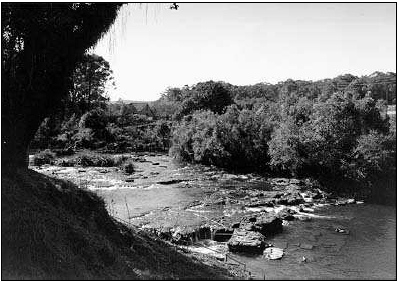
\includegraphics[width=.8\linewidth]{Imagem}
  \caption{}
  \label{histograma:sfig1}
\end{subfigure}\


\begin{subfigure}{.5\textwidth}
  \centering
  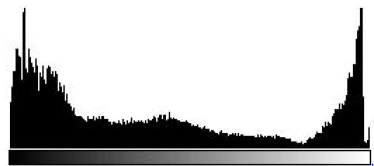
\includegraphics[width=.8\linewidth]{Histograma2}
  \caption{}
  \label{histograma:sfig2}
\end{subfigure}
\caption{(a) Uma imagem; (b)O seu histograma \cite{marques1999processamento}}
\label{HistogramaFig}
\end{figure}

    \subsection{Comparação de histogramas} \label{comparacaoHistogramas}

        Para algumas aplicações, é importante fazer comparações entre dois ou mais histogramas. Essas comparações podem revelar semelhanças ou diferença relevantes para imagens. Por exemplo, no caso desse trabalho, determinar se uma determinada região é mais semelhante a uma vaga vazia ou a um veículo qualquer. É possível também fazer essa operação para determinar eficiência de filtros ou de técnicas de normalização de histogramas.

        A comparação de histogramas consiste efetivamente em comparar duas amostras de distribuição de probabilidade. Sendo assim, várias técnicas utilizadas na área da Estatística são comumente aplicadas no Processamento de Imagens e Visão computacional. É comum se utilizar de métodos que calculam distâncias entre os diversos \textit{bins} ou seções do histograma. Um \textit{bin} é um separador que contém um intervalo dos dados que podem aparecer no histograma. Por exemplo, um histograma de uma imagem que contém 256 níveis de cinza pode possuir 256 \textit{bins} que representam um único nível de cinza cada um ou 25 \textit{bins} que representam a distribuição de um intervalo de 10 níveis de cinza cada. Comparações \textit{bin} a \textit{bin} assumem que os histogramas estão no mesmo domínio, o que normalmente não é um problema na área do Processamento de Imagens. Elas também dependem do número de \textit{bins} existentes. Se o número for pequeno, a medida da distância será robusta, mas pouco discriminativa, se for muito grande, a distância é discriminativa, mas não robusta.\cite{pele2010quadratic}

        Técnicas chamadas \textit{cross-bin}, que levam em conta diferenças além daquelas \textit{bin} a \textit{bin} existem e são bastante utilizada. Algumas delas são brevemente apresentadas em \cite{zhang2014comparison} e em \cite{rubner2000earth}. Em \cite{rubner2000earth} a técnica chamada de Distância do Movedor da Terra (\textit{Earth Mover's Distance}), derivada de comparação de grafos bipartidos e que consiste em avaliar o custo de se deslocar uma amostra - ou um histograma  - para que ela corresponda com a outra.

        Por conta das tecnologias utilizadas nesse trabalho e da natureza de sua implementação, técnicas de comparação \textit{bin} a \textit{bin} são mais interessantes do que as técnicas \textit{cross-bin}. Em particular, duas técnicas são de grande interesse para esse trabalho: a distância Qui-Quadrado e a técnica de comparação por intersecção.

        A técnica Qui-Quadrado ($\chi^{2}$) vem da área de comparação de distribuições probabilísticas onde é utilizada para testar semlhanças entre uma distribuição e as frequências observadas\cite{pele2010quadratic}.Ela dá mais importância às diferenças entre as \textit{bins} maiores do que entre as menores. Essa técnica é bastante utilizada para a classificação de objetos em imagens e identificação de imagens muito semelhantes. Ela é descrita pela fórmula:

        \begin{equation}\label{quiQuadrado}
          d(H_{1}, H_{2}) = \sum_{I = 0}^{N}\frac{(H_{1}(I) - H_{2}(I))^2}{H_{1}(I)}
        \end{equation}


        Onde $d(H_{1}, H_{2})$ é a diferença entre os dois histogramas $H_{1}$ e $H_{2}$ e $N$ é o número de \textit{bins} nos dois histogramas. Como é uma técnica de comparação entre \textit{bins}, $N$ deve ser o mesmo para os dois histogramas.

        A técnica da intersecção calcula a porção comum de dois histogramas e é particularmente útil em casos como: comparação de um mesmo objeto em ângulos de visualização diferentes, imagens com resoluções diferentes e verificação de diferenças no fundo das imagens que contém objetos. Nesse trabalho, essa técnica é utilizada para ajudar a determinar o estado das vagas no estacionamento. Esse processo é descrito na seção \ref{identificacaoFundo}.

        A diferença por intersecção pode ser descrita matematicamente como:

        \begin{equation}\label{intersecção}
          d(H_{1}, H_{2}) = \sum_{I = 0}^{N}min(H_{1}(I), H_{2}(I)
        \end{equation}

        Aonde, novamente, $d(H_{1}, H_{2})$ é a diferença entre os histogramas e $N$ é o número de \textit{bins}.


        Uma diferença importante entre as duas técnicas é que na comparação $\chi^{2}$, quanto menor o valor, mais semelhantes são os histogramas. No caso da intersecção, quanto maior o valor de $d(H_{1}, H_{2})$, maior a semelhança.

        \subsection{Equalização de histogramas} \label{equalizacaoHistogramas}

        Equalização ou normalização de histogramas é a técnica que procura redistribuir os valores percentuais de cada nível de cinza no histograma de uma determinada imagem. O objetivo é obter um histograma uniforme aonde a probabilidade de ocorrência de cada nível possível é praticamente a mesma. Utiliza-se para tal uma função de transformação aplicada sobre o histograma da imagem. A função mais comum utilizada para essa tarefa é a função de probabilidade acumulada dada por:

        \begin{equation}\label{intersecção}
          s_{k} = P(r_{k}) = \sum_{j = 0}^{k}p_{r}(r_{j})
          \caption{A equação $csf$ \cite{marques1999processamento}}
        \end{equation}

        Onde $P(r_{k})$ é o valor do nível $k$ de cinza no histograma e $p_{r}$ é a probabilidade de ocorrência deste nível na imagem e $s_{k}$ é o valor da saída.

        Aplicar técnica de equalização de histogramas é útil em diversas situações. Quando o processo é aplicado sobre uma imagem com predominância de níveis de cinza altos, tendendo ao branco, os valores se espalham por todo o espectro possível, melhorando o contraste da imagem e trazendo a tona detalhes que previamente podiam ser difíceis de se perceber.

        Quando o histograma de uma imagem escura, com valores tendendo a níveis baixos de cinza, os objetos escuros ficam mais claros e os claros ficam mais claros ainda. Apesar do aumento de claridade poder trazer perda de detalhes em seções mais claras, ele pode revelar e ajudar a detectar objetos que antes estavam escondidos em regiões muito escuras da imagem. No geral, a equalização de histogrmas tem um poder muito grande de aumentar o contraste em imagens. A figura \ref{equalizacaoHistogramasFig} demonstra esse poder de forma bastante convincente.

        Por causa disso, a equalizaçao é utilizada extensivamente em diversas áreas do Processamento de Imagens. Na medicina, pode ajudar médicos a fazerem diagnósticos melhores ao analisarem imagens médicas. Realçar fotos antigas que perderam o contraste também é uma tarefa que pode ser cumprida com essa técnica.

        É possível também executar a equalização do histograma de apenas uma parte da imagem. Isso serve no geral para realçar detalhes da imagem que podem ser mais interessantes que a imagem como um todo. Nesse trabalho, o histograma de trechos da imagem aonde se sabe que existe uma vaga de um estacionamento e se desconfia que um veículo estacionou é equalizado e comparado com um histograma de controle, como detalhado na seção \ref{identificacaoFundo}. Essa equalização, porém, é feita no histograma da imagem no espaço HSV de imagens e tem a função principal de preparar estes histogramas para as técnicas de comparação descritas na seção \ref{comparacaoHistogramas}.


        \begin{figure}
      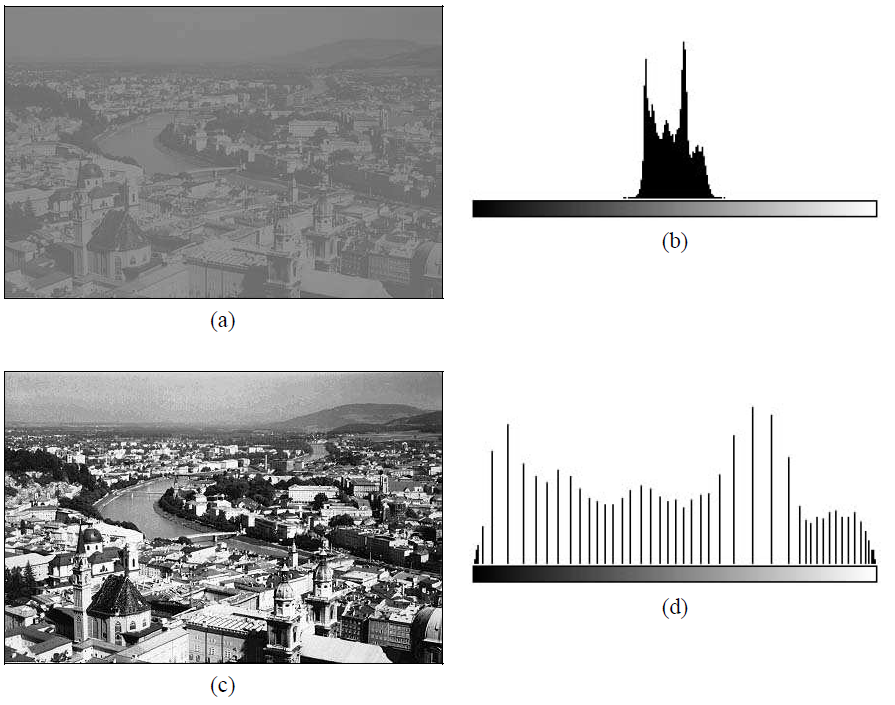
\includegraphics[width=1\textwidth]{equalizacaoHistograma}
      \caption{Aplicação da equalização de histograma a uma figura de baixo contraste. (b) mostra o histograma de (a) e (d) mostra o histograma de (c) \cite{marques1999processamento}}\label{equalizacaoHistogramasFig}
    \end{figure}










    \section{Segmentação de objetos} \label{segmentacao}
        Um processo importante para vários sistemas de visão computacional é o da extração de características ou \textit{features} importantes de uma ou mais imagens. Através destes \textit{features}o computador deve ser capaz de extrair uma informação ou conhecimento desejado, ou até mesmo mostrar na saída uma imagem diferente que possa ser analisada por humanos a fim de determinar essa informação.

        Quando o objetivo do processo é de localizar e extrair a posição de objetos específicos em uma cena, chamamos esse processo de segmentação de objetos. Ele consiste basicamente em isolar e selecionar \textit{pixels} da imagem de entrada que possam fazer parte da representação visual do objeto\cite{graciano2007rastreamento}. A saída desses programas pode ser uma imagem que contem apenas os objetos desejados, ou um arquivo com informações como o número de objetos encontrados diferentes encontrados.

        Existem diversas técnicas para segmentação de objetos descritas na literatura. Cada uma dessas técnicas é ideal para um tipo diferente de imagem ou de objeto a se encontrar. Assim como em muitas áreas da computação, a decisão da técnica a ser utilizada é tão importante quando a implementação do programa propriamente dito.

        É interessante apresentar alguns conceitos importantes antes de iniciar uma discussão sobre técnicas de segmentação. O primeiro deles é o conceito de vizinhaça do \textit{pixel}. A vizinhança de um ponto de uma imagem é um objeto de estudo importante para determinar objetos. Ela consiste essencialmente dos valores dos \textit{pixels} ao redor do \textit{pixel} sendo analisado. Chamamos de vizinhança-4 o conjunto dos quatro \textit{pixels} que ficam diretamente acima, abaixo, à direita e à esquerda do ponto em questão. A vizinhança-8, por sua vez, é então o conjunto que consiste da vizinhança-4 e mais os quatro \textit{pixels} nas diagonais do ponto sendo analisado. Chamamos os \textit{pixels} que fazem parte de alguma vizinhança de outro \textit{pixel} de vizinho.

        O segundo conceito importante é a definição de bordas. As bordas em uma imagem representam os limites de cada objeto e são, portanto, de extrema importância na segmentação de objetos em imagens. Pontos pertencentes a bordas são aqueles que possuem uma mudança brusca nos níveis de cinza. Por exemplo, podemos definir um ponto de uma borda em uma imagem binária - que possui apenas pontos brancos ou pretos - como um ponto preto que contenha pelo menos um vizinho branco.\cite{vkl1989jain}

        Uma técnica simples e muito utilizada para segmentação é da limiarização, ou \textit{thresholding}. Essa técnica consiste na categorização dos \textit{pixels} de uma imagem através de um limiar \textit{L}. Aqueles que possuirem valores maiores que \textit{L} terão seu valor configurado como o valor máximo, representado pela cor branca. Normalmente o valor do limiar é escolhido de acordo com a expectativa dos valores de cinza dos obejtos do conjunto de interesse da imagem, mas é possível também implementar formas de detectar um limiar apropriado computacionalmente. Na seção \ref{segmentacaoVeiculos} é descrito como o histograma de cada quadro foi usado para determinar um limiar global para a execução do \textit{thresholding} de cada \textit{frame}. O resultado é visível na figura \ref{LimiarizacaoFig}. É possível também, e apropriado em vários casos, determinar limiares locais para a imagem. Nesse caso, cada fragmento da imagem, como um quadrante, possui um valor diferente de \textit{L}. O resultado desse processo de limiarização é normalmente uma imagem binária.


\begin{figure}
 \centering
\begin{subfigure}{.5\textwidth}
  \centering
  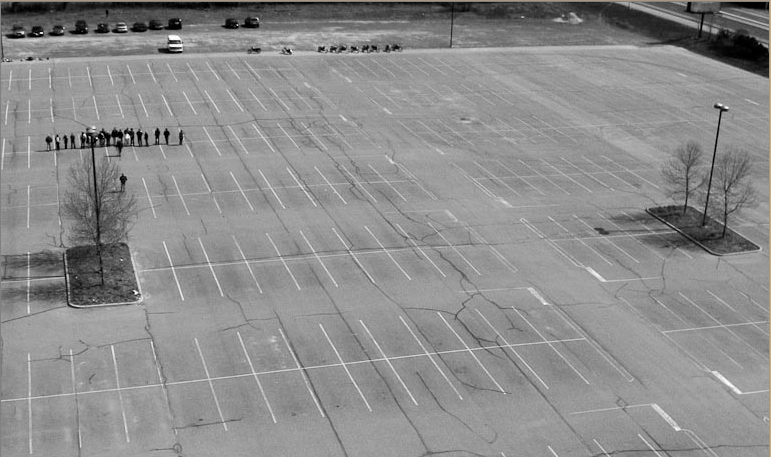
\includegraphics[width=.8\linewidth]{Estacionamento}
  \caption{}
  \label{Limiarizacao:sfig1}
\end{subfigure}\


\begin{subfigure}{.5\textwidth}
  \centering
  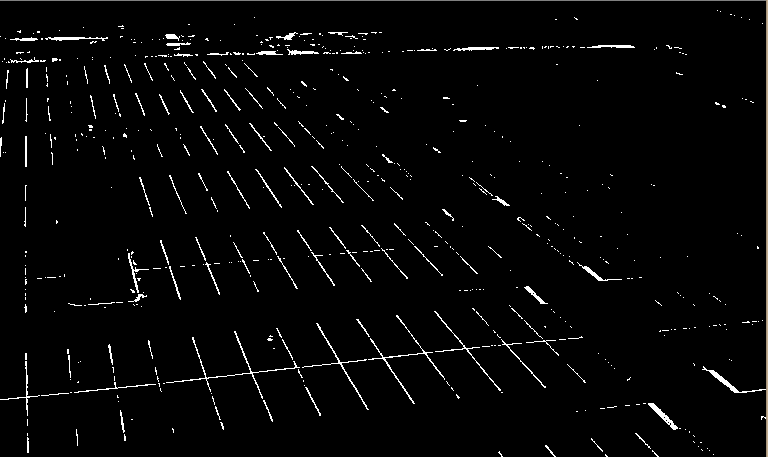
\includegraphics[width=.8\linewidth]{EstacionamentoBinarizado}
  \caption{}
  \label{Limiarizacao:sfig2}
\end{subfigure}
\caption{(a) Uma imagem de um estacionamento; (b) A mesma imagem binarizada através da técnica utilizada na seção \ref{segmentacaoVeiculos}}
\label{LimiarizacaoFig}
\end{figure}

    Uma vez que temos uma imagem binarizada podemos utilizar várias técnicas para separar os objetos. A mais simples de todas, nos casos onde a imagem contém apenas um objeto de interesse que possui valores brancos na imagem, podemos simplesmente encontrar todos os \textit{pixels} brancos. Em imagens binárias que possuem mais de um objeto de interesse é preciso implementar uma maneira de se separar esses objetos. Existem técnicas que analisam a conectividade dos pontos a fim de extrair limites dos objetos.\cite{vkl1989jain} Outros algoritmos classificam pontos com o valor de interesse em classes diferentes. Pontos com o valor interessante não-classificados que sejam vizinhos de um ponto de uma classe passam a fazer parte daquela classe ou passam a integrar uma classe nova caso contrário. Ao final da execução, cada classe contém os \textit{pixels} de um objeto diferente.

    Outra técnica interessante de separação de objetos em imagens é o algoritmo chamado \textit{watershed}. \textit{Watersheding} é um algoritmo morfológico que permite a detecção de bordas em imagens em níveis de cinza. É uma técnica muito eficiente e que produz contornos bastante precisos. Esse algoritmo possue uma desvantagem particular em relação a outros algoritmos de segmentação de imagens. Por vezes, se mal utilizado a técnica de \textit{watersheding} pode segmentar demais a imagem, reconhecendo objetos não existentes. Existem então, diversas pesquisas para minimizar esse problema, como a apresentada em \cite{malpica1997applying}.

    O algoritmo de \textit{watershed} consiste em interpretar a imagem como um mapa topológico de uma região, onde os pontos mais escuros representam pontos mais baixos, ou "vales". Uma vez detectados esses vales, o algoritmo começa um processo de inundação do vale, daí o nome. Computacionalmente, esse processo de inundação consiste na atribuição de classes a pixels adjacentes ao vale que se propaga a cada iteração. Os pontos onde a água se encontraria - ou pontos que seriam atribuídos a duas classes - são os pontos de borda da imagem. Essa técnica é muito usada no ramo da Biologia, para a segmentação de células em imagens de microscópio.

    É importante também diferenciar objetos encontrados em uma imagem um do outro. Muitas vezes a imagem binária resultante de um processo de segmentação contém diversos objetos. Em alguns casos, não temos interesse em todos eles e é importante que o computador seja capaz de diferenciar um do outro. Existem diversas técnicas que visam esse objetivo. É possível analisar o histograma apenas da região onde o programa sabe que existe um objeto e comparar com um histograma esperado. Outros algoritmos se utilizam de operações matricias que se aproximam de uma derivação a fim de encontrar a orientação das bordas do objeto do objeto detectado.

    Outra abordagem bastante utilizada é a de redes neurais treinadas para identificar esses \textit{features} de objetos de interesse. Objetos encontrados são analisados por uma técnica qualquer e suas características são encontradas. As redes são então treinadas para classificar objetos com as mesmas características junto com os seus semelhantes. Esse tipo de implementação já foi utilizada com sucesso em aplicações para gerenciamento de estacionamento, como a apresentada em \cite{true2007vacant}.

    Para a implementação programa apresentado nesse trabalho são de particular interesse as técnicas de segmentação baseadas em \textit{thresholding} e subtração de fundo. As técnicas de geração e subtração de fundo serão descritas mais adiante na seção \ref{background}. Além delas, as técnicas de reconhecimento de \textit{features} de objetos através de comparação de histogramas serão bastante utilizadas para a confirmação de que o objeto encontrado é um veículo.

    \section{Subtração de imagens}  \label{subtracao}

    A diferença entre duas imagens pode ser obtida através de uma subtração simples dos valores dos elementos da primeira imagem com os elementos correspondentes da segunda imagem. Matematicamente podemos expressar essa operação pela equação:
    \begin{equation}
        D(x,y) = A(x,y) - B(x,y)
    \end{equation}

    Onde $D(x,y)$, $A(x,y)$ e $B(x,y)$ são os valores dos \textit{pixels} na posição (x,y) das imagens de diferença obtida e as imagens A e B originais. Podemos subtrair imagens RGB fazendo a subtração normal de cada canal da primeira imagem com o canal correspondente da segunda.

    A grande utilidade de se subtrair duas imagens é justamente realçar as diferenças entre estas duas imagens. Obter a diferença de duas imagens pode ser útil para facilitar a visualização de resultados da aplicação de uma algoritmo ou para encontrar mudanças que ocorrem entre dois quadros distintos de um vídeo capturado. A diferença entre dois quadros de um vídeo contém a posição de um objeto que se moveu na cena, mais o ruído da imagem. Essa segunda aplicação mencionada é de grande relevância para este trabalho. Na seção \ref{segmentacaoVeiculos} mais a frente, eu descrevo como utilizei a diferença entre dois quadro consecutivos para encontrar uma região que contenha um veículo em movimento, e na seção \ref{geracaoFundo} mostro como utilizei essa região para separar dinamicamente o \textit{background} da imagem dos elementos de \textit{foreground}. Além disso, no algoritmo descrito na seção \ref{diferencasFundos} utilizo a diferença entre o fundo da imagem em dois momentos diferentes para detectar veículos que estacionaram nesse período de tempo e passaram a fazer parte do fundo.

    Se uma imagem composta por valores de níveis de cinza tem o valor de cada um dos seus \textit{pixels} representado por 8 bits, os valores que podem ser representados estarão então entre o intervalo de 0-255. Mas imagens resultantes da subtração de outras duas imagens terão seus valores representados na faixa de -255 a 255. É preciso então processar esses valores para trazê-los de volta para o intervalo que podemos representar. Existem diversas soluções para esse problema. Os algoritmos deste trabalho, porém, se importam apenas com a existência de uma diferença entre duas imagens e a posição dos \textit{pixels} que possuem valor maior que zero na imagem de diferença e não os valores específicos de cada um. Sendo assim, a abordagem utilizada para resolver essa situação foi apenas a extração do valor absoluto do resultado da diferença.

    A figura \ref{SubtracaoFig} ilustra a subtração de duas imagens. O resultado apresentado já passou por um processo de limiarização e portanto é uma imagem binária. As imagens utilizadas são fundos gerados dinamicamente. A imagem obtida pela subtração mostra uma diferença em uma região onde é sabido que há vagas no estacionamento. Na seção \ref{diferencasFundos} é descrito como essa informação é utilizada para determinar que um carro estacionou em uma vaga.

    %Colocar uma imagem de subtração de imagens%


    \begin{figure}
 \centering
\begin{subfigure}{.5\textwidth}
  \centering
  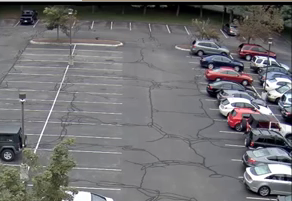
\includegraphics[width=.5\linewidth]{FigSubtracao1}
  \caption{}
  \label{Subtracao:sfig1}
\end{subfigure}%
\begin{subfigure}{.5\textwidth}
  \centering
  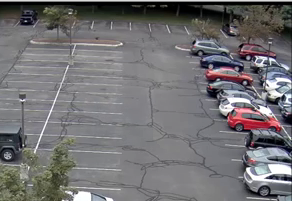
\includegraphics[width=.5\linewidth]{FigSubtracao2}
  \caption{}
  \label{Subtracao:sfig2}
\end{subfigure}


\begin{subfigure}{.5\textwidth}
  \centering
  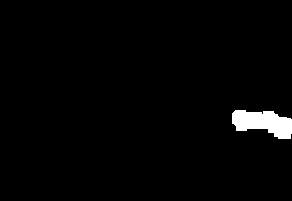
\includegraphics[width=.8\linewidth]{FigSubtracao3}
  \caption{}
  \label{Subtracao:sfig3}
\end{subfigure}
\caption{(a) O fundo em um determinado quadro em um vídeo; (b) O fundo em um outro quadro do mesmo vídeo alguns segundos depois; (c) A imagem resultante da subtração entre (a) e (b) binarizada.}
\label{SubtracaoFig}
\end{figure}



    \section{Operações Morfológicas} \label{morfologicas}
    O principio básico da morfologia matemática consiste em extrair as informações relativas à geometria e à topologia de um conjunto desconhecido (uma imagem), pela transformação através de outro conjunto completamente definido, chamado elemento estruturante.\cite{marques1999processamento} Para aplicar operações morfológicas então, precisamos primeiramente definir conjuntos sobre as imagens. Normalmente aplicamos as operações descritas a seguir em imagens binárias e essas imagens podem ser descritas completamente pelo conjunto A definido por:

    \begin{equation}\label{conjuntoA}
      A = {(x,y)|P(x,y) > 0}
    \end{equation}

    Ou, mais simplesmente, o conjunto dos \textit{pixels} $P(x,y)$ que não são pretos.

    O elemento estrutrante $B$ para as operações morfológicas é uma segunda matriz, de tamanho geralmente menos do que o da imagem original que deve ser escolhida cuidadosamente para que se obtenha os resultados desejados.

    As duas operações morfológicas básicas para o Processamento de imagens são: a dilatação, que aumenta os elementos de uma imagem alterando a área ao redor de um determinado \textit{pixel} para conformar a um dado padrão e a erosão, que se utiliza do elemento estruturante para remover objetos indesejados e diminuir elementos.\cite{de2006introduccao}.

    A dilatação faz com que um objeto presente na imagem cresça de tamanho. Ela é utilizada também para elminiar buracos em componentes segmentados, pois falhas menores do que o elemento estruturante B são completamente cobertas ao final da operação. Se chamarmos o conjunto de todos os pontos da imagem de $I$, podemos definir o conjunto resultante da operação de dilatação como:


    \begin{equation}\label{conjuntoDilatacao}
      D(A,B) = A \oplus B = \{{(x,y) \in I | B_{(x,y)} \cap A \neq \emptyset}\}
    \end{equation}

    Isto é, todos os elementos de $I$ aonde $B$, se deslocado para a posição (x,y) do elemento, intercepta o conjunto dos pontos brancos, $A$. A figura \ref{DilatacaoFig} ilustra o resultado do processo de dilatação.

    \begin{figure}
 \centering
\begin{subfigure}{.5\textwidth}
  \centering
  
\includegraphics[width=.4\linewidth]{ADilatar}
  \caption{}
  \label{Dilatacao:sfig1}
\end{subfigure}%
\begin{subfigure}{.5\textwidth}
  \centering
  
\includegraphics[width=.2\linewidth]{Elementoestruturante}
  \caption{}
  \label{Dilatacao:sfig2}
\end{subfigure}


\begin{subfigure}{.5\textwidth}
  \centering
  
\includegraphics[width=.4\linewidth]{Dilatada}
  \caption{}
  \label{Dilatacao:sfig3}
\end{subfigure}
\caption{(a) Uma imagem binária; (b) O elemento estrutrante a ser utilizada na dilatação; (c) A imagem resultando do processo de dilatação, com os pixels adicionados pintados de azul para facilitar a visualização}
\label{DilatacaoFig}
\end{figure}


    Nesse trabalho, a dilatação é utilizada na seção \ref{segmentacaoVeiculos} para aumentar a área da mancha encontrada pela diferença dos quadros consecutivos, a fim de determinar uma maior área que certamente pertence ao \textit{foreground}.

    A erosão por sua vez faz o processo contrário da erosão. Ela dimunui o contorno dos objetos, pode diminuir o número de componentes segmentados e até remover elementos que sejam menores do que o elemento estruturante, uma vez que componentes que sejam menores serão eliminados da imagem $I$. Uma aplicação interessante da operação de erosão é na detecção de contornos. Podemos subtrair uma imagem de sua versão erodida para encontrar os contornos dos objetos presentes na imagem.

    Da mesma forma que com a dilatação, podemos definir a erosão matematicamente como:

    \begin{equation}\label{conjuntoErosao}
      D(A,B) = A \ominus B = \{{(x,y) \in I | B_{(x,y)} \subseteq A}\}
    \end{equation}

    Ou seja, os pontos em $I$ tais que o elemento estruturante $B$ deslocado para a posição (x,y) do ponto, está contido completamente em A. Mais especificamente, apenas os pontos onde se sobrepusermos o $B$ só haverá pontos brancos sob os pontos de B. A figura \ref{ErosaoFig} ilustra o processo de erosão sobre uma imagem binária.

       \begin{figure}
 \centering
\begin{subfigure}{.5\textwidth}
  \centering
  
\includegraphics[width=.4\linewidth]{ADilatar}
  \caption{}
  \label{Erosao:sfig1}
\end{subfigure}%
\begin{subfigure}{.5\textwidth}
  \centering
  
\includegraphics[width=.2\linewidth]{Elementoestruturante}
  \caption{}
  \label{Erosao:sfig2}
\end{subfigure}


\begin{subfigure}{.5\textwidth}
  \centering
  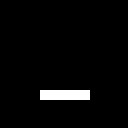
\includegraphics[width=.4\linewidth]{Erodida}
  \caption{}
  \label{Erosao:sfig3}
\end{subfigure}
\caption{(a) Uma imagem binária; (b) O elemento estrutrante a ser utilizada na erosão; (c) A imagem resultando do processo de erosão}
\label{ErosaoFig}
\end{figure}

    É possível também combinar essas operações entre si para criar novas operações morfológicas sobre as imagens. As combinações mais comuns formam as operações de abertura e fechamento. A abertura é a aplicação de uma dilatação seguida de uma erosão. A operação da abertura suaviza os contornos dos objetos na imagem, ou seja, ela remove pequenas protuberâncias. O fechamento por sua vez, é a combinação de uma erosão seguida de uma dilatação. Essa operação é utilizada para fechar pequenos buracos ou falhas contidos no interior de um objeto na imagem binária.


   \section{Geração de background} \label{background}

   Uma área de estudos de muita utilidade na segmentação de objetos é de geração de fundo. Em particular, segmentar os objetos que pertencem ao \textit{foreground} dos objetos que pertencem ao fundo da imagem é uma etapa crucial nos programas de segmentação ou rastreamento de objetos em vídeo. De fato, o primeiro passo nesses algoritmos normalmente é encontrar um fundo para servir de imagem de referência e possibilitar que sejam aplicadas técnicas de subtração de fundo com a finalidade de encontrar objetos que estejam em movimento.

   A abordagem típica de determinação de \textit{background} é obter a imagem de referência para o fundo quando a cena está estática.\cite{shoushtarian2003practical}. Na prática essa abordagem não é totalmente eficiente, principalmente em aplicações que dependem de imagens obtidas de câmeras de segurança ou de ambientes que não costumam ficar totalmente sem movimento. Em programas que obtém as imagens através de câmeras que filmam o mesmo ambiente durante um dia inteiro, mudanças na iluminação, tanto natural quanto artificial, modificam o fundo da imagem. Além disso, objetos que estavam em movimento podem se tornar objetos estáticos e devem ser agregados ao \textit{background}.

   É preciso então encontrar técnicas para determinar o fundo da imagem em tempo de execução, de forma adaptativa e dinâmica. Alguns programas se utilizam da média aritmética ou dos quadros durante o decorrer do vídeo. Similarmente a observar apenas uma imagem, pode-se observar a mediana dos valores de cada \textit{pixel} dos quadros. O algoritmo apresentado em \cite{shoushtarian2003practical} se utiliza de temporizadores para atualizar os valores dos pixels de fundo e em \cite{chen2012dynamic} é apresentado ainda um outro método.

   Esse trabalho se utiliza de uma técnica de geração de fundo similar àquela apresentada em \cite{hai2009self} que provou ter grande sucesso na determinação de imagens de fundo em câmeras de monitoramento de trânsito. O algortimo é descrito com mais detalhes na seção \ref{geracaoFundo}.



    \section{Espaços de cor} \label{espaçosCor}

    A percepção de cor não é nada mais do que uma reação gerada no sistema visual humano quando a luz estimula as células presentes na retina. Dentre essas células, as importantes para a representação e interpretação de imagens são os cones, dos quais existem três tipos. Essas células são responsáveis pela interpretação de cor no olho humano. Como existem exatamente três tipos diferentes de cones, podemos descrever uma cor com exatamente três componentes numéricos, desde que apropriadamente ponderados.\cite{plataniotis2000color}. Um modelo de representação de cores é chamado de um espaço de cor.

    Antes de apresentar os espaços de cor relevantes ao trabalho, é interessante definir alguns conceitos importantes:

    \begin{itemize}
       \item O brilho (Br) é o atributo que define a sensação visual de que uma determinada área de uma imagem emite mais ou menos luz.
       O brilho de uma imagem é parcialmente responsável pela seu valor de luminosidade (L).
       \item A matiz da cor(Hue ou H) é o valor associado ao comprimento de onda predominante de uma determinada cor. A visão humana se utiliza principalmente deste atributo para diferenciar e identificar cores. Quando falamos que um objeto é vermelho, verde ou amarelo, normalmente estamos falando da matiz da cor do objeto.
       \item A saturação (S) se refere a "pureza" da cor ou ao quanto a matiz da cor está intocada. Em termos formais, a saturação é inversamente proporcional a quantidade de luz branca misturada a matiz.
     \end{itemize}

     Existem diversos espaços de cor diferentes. Alguns baseados em especificações de dispositivos, outros que visam simular a percepção real de cores e alguns que procuram separar valores importantes na representação da imagem. Cada um deles tem uma aplicação distinta. Nesse trabalho dois espaços são mais relevantes: o espaço RGB e o espaço HSV.

     \subsection{O espaço RGB}\label{RGB}

     RGB é um acrônimo para \textit{Red, Green, Blue}, vermelho, verde e azul em inglês. Essas são cores primárias que quando adicionadas corretamente podem gerar qualquer outra cor. Nesse espaço, a cor de cada \textit{pixel} em uma imagem é representada por um vetor de três coordenadas onde cada uma representa a quantidade de uma das três cores presentes no \textit{pixel}. Sendo assim, ele é considerado um sistema aditivo.

     O espaço RGB é o mais conhecido e provavelmente mais popular dos espaços de cor. Ele é uma escolha muito comum para representação digital de imagens, já que a maioria dos dispositivos de saída de imagem se utilizam da adição do vermelho, verde e azul para gerar as cores desejadas em cada \textit{pixel}. Por causa disso, utilizar o formato RGB traz diversas vantagens no quesito de arquitetura e elaboração de um sistema.

     O espaço RGB pode ser interpretado como um cubo, aonde os três eixos correspondem ao valor de vermelho, verde e azul.  O vértice no canto inferior aonde o valor de cada cor é 0 representa o preto, e o vértice oposto a ele representa o branco.\cite{ford1998colour} A diagonal que liga esses dois vértices representa então diversos níveis de cinza.

     Esse espaço apresenta algumas desvantagens. Uma delas é que no geral ele é dependendte do dispositivo sendo utilizado. Isto é, monitores diferentes apresentam discrepâncias ao mostrar imagens que têm os mesmo valores RGB em cada pixel. Além disso, ele não é muito ideal para representação de imagens reais, como fotografias ou imagens impressas. Isso é porque para formar corretamente uma cor cada componente RGB deve estar dentro da mesma largura de banda. Mas o maior problema com o espaço RGB para processamento de imagens é que ele traz algumas dificuldades para o processamento. Por exemplo, se um programa quer modificar a cor de uma determinado parte de uma imagem ou aumentar a intensidade luminosa de um \textit{pixel}, todos os três valores RGB devem ser recuperados e modificados apropriadamente um a um e depois atualizados. Sendo assim, para muitas aplicações em visão computacional, uma transformação do espaço RGB, chamada HSV, descrita na subseção \label{HSV} é utilizada.

     \subsection{O espaço HSV}\label{HSV}

     O espaço de cores HSV (\textit{Hue, Saturarion, Value} ou Matiz, saturação e valor) é um espaço de cores feito para ser mais intuitivamente legível para humanos. Como definimos as cores principalmente através dos valor de matiz e saturação, esse espaço se aproveita disso para representar cores de uma forma que seja mais fácil e intuitivo de se escolher uma cor do que no RGB. O atributo \textit{value} se refere a uma medida de luminosidade do ponto.

     Esse espaço não é nada mais da que uma deformação do cubo RGB e pode-se transformar facilmente uma imagem entre um formato e outro. De fato, os algoritmos são simples e todas as bibliotecas especializadas fornecem funções próprias para essa transformação. Ele é representado através de um círculo ao redor da linha diagonal que liga os vértices que representam o preto e o branco no cubo RGB. A posição do círculo nessa reta indica a luminosidade do ponto, enquanto a matiz é representada por um ângulo no círculo e a saturação pela distância radial do eixo de luminosidade para a cor. A figura \ref{figConeHSV} mostra uma representação visual destes conceitos.
     
     \begin{figure}
     \centering
      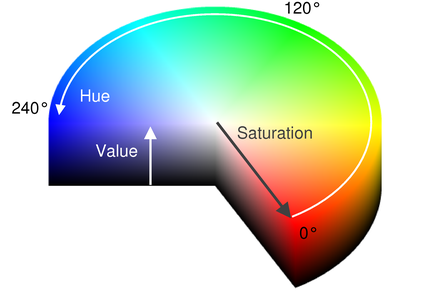
\includegraphics[width=.5\textwidth]{hsv}
      \caption{Representação visual do funcionamento do espaço de cor HSV}\label{figConeHSV}
    \end{figure}

     
     Tratar imagens no espaço HSV traz várias facilidades. É possível mudar os atributos da imagem ou de uma pequena seção da imagem modificando apenas um valor. Por exemplo, se uma aplicação deseja modificar as cores de uma imagem, basta recuperar os valores da matiz de cada ponto de cor e modificá-lo em uma certa quantidade de graus. Porém, como ele não passa de uma transformação do espaço RGB, a maioria das desvantagens apresentadas na subseção \ref{RGB} continuam presentes.

     Porém, a importância desse espaço de cor no processamento de imagens não vêm da capacidade intuitiva de se escolher uma determinada cor. Ele é muito relevante porque separa as informações de cor e luminosidade em cada ponto da imagem. Essa separação é muito importante para diversas aplicações. Ao equalizar histogramas por exemplo, é recomendado que o processo seja aplicado sobre o canal de luminosidade da imagem. Isso evita que as cores da imagem sejam modificadas de forma exagerada. Outra situação relevante é a de sombras ou outras mudanças de iluminação em reconhecimento de objetos ou regiões conhecidas. Quando uma área ou objeto está sobre algum efeito de iluminação, normalmente a maior modificação é no componente de luminosidade do ponto, enquanto a matiz da cor continua inalterada. Isso permite o reconhecimento de objetos ou de semelhanças mesmo sobre condições de iluminação diferentes. Por isso esse trabalho se utiliza do componente H de trechos de imagens para a comparação de histogramas na seção \ref{testesEstaticas}.
     
     \section{Classificação de objetos} \label{classificacao}
     
     Classificação de objetos em imagens consiste no agrupamento de objetos que foram vistos pelo sistema em classes diferentes. Esse processo se assemelha bastante ao reconhecimento de objetos em imagens. De fato, pode-se argumentar que reconhecer objetos individualmente é uma forma de classificar objetos aonde cada objeto compõe uma classe diferente.
     
     Objetos podem ser classificados com relação a várias características como cor predominante, tamanho, forma e muitas outras. Normalmente se escolhe parâmetros que sejam independentes entre as classes e diferenciem suficientemente objetos de classes distintas. O processo em si normalmente é feito se utilizando de alguma forma de rede neural. Uma vez determinados os parâmetros a serem utilizados, um conjunto de treinamento é criado.
    
     Para criar o conjunto inicial de imagens de treinamento para a rede neural responsável pela classificação, assume-se que o desenvolvedor esteja munido de uma aplicação capaz de detectar os atributos relevantes nas imagens. Quando esse é o caso, esse programa é expostos a diversas imagens contidas nas diferentes classes que se deseja separar. Ele determina os atributos presentes na imagem e então um usuário atribui aquela imagem a uma das classes. O programa então armazena a distribuição de valores para cada atributo através das imagens.  O passo seguinte é determinar um ponto de separação de cada classe para cada um dos atributos. Uma vez que os valores de atributo associados a cada classe são determinados, o programa é exposto a um conjunto de testes. A partir das informações obtidas na etapa de treinamento, o programa é capaz de classificar os objetos em uma imagem com sucesso.
     
     Por exemplo, suponha que um desenvolvedor queira elaborar um sistema que diferencia laranjas de limões. Uma possível solução é o uso da classificação de objetos em imagens. Para isso, o desenvolvedor iria expor seu programa a centenas de imagens de laranjas e de limões. As imagens de laranja são predominantemente laranjas, enquanto as de limão são predominantemente verdes. Esses então são atributos ideiais para a classificação. Esse programa então iria elaborar uma distribuição dos valores de laranja e verde de cada imagem exibida a ele. Munido dessa distribuição, basta determinar um limiar que separe as duas cores suficientemente. Dessa forma, se o valor de uma dessas cores está acima dessa limiar, é muito provável que a imagem seja da fruta correspondente à cor. Assim, o programa é capaz de distinguir entre imagens de laranjas e limões.
     
     
    


    
  \chapter{Metodologia} \label{Metodologia}


\section{Tecnologias Utilizadas} \label{tecnologiasUtilizadas}

    Para a implementação deste trabalho, foi utilizada a biblioteca OpenCV, versão 2.4.8. Essa biblioteca desenvolvida pela Intel dá acesso a várias funções importantes para Processamento de imagens e Visão computacional em diversas linguagens como C++, Python e Java. Nesse trabalho a linguagem escolhida foi o C++. Foi escolhida a versão 2.4.8 ao invés da mais recente 3.0.0 pela sua consistência e facilidade de instalação, além de uma documentação mais completa.
    
    A IDE utilizada foi a Microsoft Visual Studio 2015 versão Community. Essa IDE foi escolhida por causa da grande facilidade que traz para a instalação de bibliotecas externas como a OpenCV utilizada no trabalho e também por causa da possibilidade de se instalar diversos plugins que podem facilitar o desenvolvimento, como o Image Watch, plugin que permite a visualização das imagens geradas pelo programa em grande detalhe.

%Seçao sobre como obti as imagens para os testes do trabalho ---- a maquete/o drone.




\section{Segmentação dos veículos} \label{segmentacaoVeiculos}

    A primeira etapa na implementação do programa apresentado nesse trabalho é a da segmentação dos veículos em movimento durante o decorrer do vídeo obtido pela câmera estática. Para detectar esse veículos, esse projeto utiliza uma técnica de segmentação baseada naquela apresentada em \cite{hai2009self}. Segmentar corretamente os carros é crucial para o procedimento descrito na seção \ref{geracaoFundo}. Nessa seção, descrevo como uma imagem com apenas o contorno de um carro é obtida.

    Primeiramente, é extraída a imagem de diferença entre dois quadros consecutivos. Chamamos essa imagem de \textit{D}. Essa diferença é trivial, nada mais é do que o valor absoluto da diferença entre o valor do mesmo \textit{pixel} em cada um dos dois quadros. Pixels que representam objetos que se mantiveram estáticos durante os dois quadros originais, como o asfalto e carros estacionados, devem ter então valor zero em \textit{D}. Portanto, é de se esperar que a imagem \textit{D} tenha uma grande quantidade de valores próximos ou iguais a zero.

    Após extraída a diferença entre os dois quadros, resta binarizar \textit{D}. Como descrito na seção \ref{segmentacao}, é preciso encontrar um limiar apropriado para cada imagem de diferença obtida. Como elas são obtidas dinamicamente, determinar esse limiar de forma estática, não traz resultados satisfatórios. Pares de quadros que apresentam menos movimento possuem valores de diferença menores e portanto, as regiões que devem ser tornadas brances têm valores inicialmente mais baixos.

    Sabendo que a grande maioria dos pixels de \textit{D} possui valor próximo a zero, podemos determinar um limiar \textit{T} de forma dinâmica. Para encontrar o valor ideal de \textit{T}, o programa primeiro encontra o pico do histograma de \textit{D}. O nível de cinza correspondente a esse valor é o que mais ocorre na imagem e será sempre um valor bem próximo de zero. O valor escolhido para \textit{T} é o terceiro nível de cinza cujo valor no histograma é inferior a 1\% do valor do pico. A escolha desse valor ao invés do primeiro vem de um problema gerado por ruído na captura da imagem.

    Por conta de ruído na imagem, valores de pixels em pontos estáticos, como por exemplo, parte do asfalto, apresentam pequenas diferenças que poluem a imagem de diferença. Esses pequenos pontos com difereça maior que zero podem aparecer na imagem binarizada, gerando regiões indesejadas. Para minimizar esse problema, duas medidas são tomadas. A primeira é a aplicação do parâmetro do limiar mínimo \textit{lm}. Esse valor depende do vídeo sendo analizado e deve ser maior quanto maior for o ruído da câmera. Antes do cálculo do histograma da imagem de diferença o programa configura todos os valores abaixo desse limiar para o valor mínimo. Isso desvia o histograma para valores menores e gera uma binarização mais limpa. A determinação correta de \textit{lm} é essencial para uma boa segmentação. A segunda medida é a escolha do terceiro valor inferior a 1\% do pico. Isso evita apenas que o ruído não seja responsável ao acaso pelo limiar escolhido estar abaixo do desejado. A figura \ref{fig:Diferenca} mostra o resultado do processo.

    \begin{figure}[h]
      \centering
      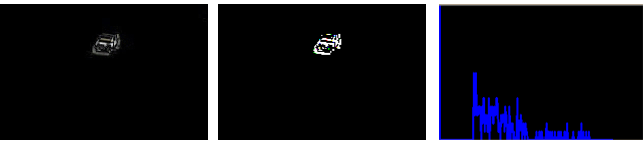
\includegraphics[width=\textwidth]{FiguraDiferenca}
      \caption{A esquerda: a imagem de diferença D. Ao centro: D binarizada com a técnica descrita acima. A direita: o histograma de D}\label{fig:Diferenca}
    \end{figure}

\section{Rastreamento dos veículos} \label{rastreamentoVeiculos}
    
      A técnica de segmentação de veículos apresentada na seção \ref{segmentacaoVeiculos} provê resultados parciais que podem ser utilizados e processados para se atingir obter diversas informações. Uma possibilidade é a geração de fundo dinâmica apresentada na seção \ref{geracaoFundo}. O outro tratamento que esse programa dá para as imagens obtidas na seção \ref{segmentacaoVeiculos} é rastrear os objetos que estão em movimento no vídeo através do acompanhamento das diferenças entre quadros.
      
      Para cada imagem $D$ binária obtida quando se faz a diferença entre dois quadros do vídeos, o programa procura os contornos de todas as manchas brancas presentes na imagem e os armazena em um vetor. Em seguida, o progrma calcula o menor círculo que contém completamente cada um desses contornos e armazena os seus centros em um vetor $C$ de coordenadas.
      
      O programa possui ainda uma estrutura de Rastro, que possui duas coordenadas: a do início e o fim do rastro. Uma vetor $R$ de rastros armazena cada rastro que está ainda sendo computado pelo programa.
      
      Munido de $R$, $C$ e a imagem $D$ gerada pela diferença entre os quadros, o programa passa a analisar de quais rastros cada centro faz parte. Ele percorre o vetor de $C$ de centros dos contornos e o compara com as coordenadas dos finais de cada rastro em $R$. Se $R$ estiver vazio, um novo rastro é criado com início no centro que está sendo analisado e final provisoriamente populado com o valor de coordenada igual ao do ínicio. Caso contrário, o programa verifica se o centro analisado $c$ atende as seguintes condições em relação ao final de um determinado rasto $f_{R}$:
      
      \begin{itemize}
        \item Distância Máxima: A coordenada de $c$ a uma distância menor da coordenada de $f_{R}$ do que uma distância máxima determinada manualmente. Essa distância é calculada utilizando um método de distância euclidiana simples, apresentado na equação \ref{distanciaEuclidiana}. Se $c$ não cumpre essa condição, o programa considera imediatamente que ele não deve fazer parte da rastro em questão.
        \item Ângulo entre vetores: Para evitar que um veículo que passa muito próximo a outro em sentido oposto "tome conta" do seu rastro, o ângulo vetorial entre $c$ e $f_{R}$ é calculado. Novamente, ele não pode ultrapassar um limiar imposto manualmente.
        \item Direção predominante das bordas: Os contornos em $D$ possuem bordas que podem ser analisadas para determinar direção, usando uma multiplicação matricial que se assemelha a operação da derivada. Essa terceira condição tem o papel apenas de complementar a segunda.
      \end{itemize}
      
      Se $c$ atende às condições listadas acima para o final de algum rastro, $c$ passa a ser o final daquele rastro e o programa passa para o próximo contorno a ser analisado.
      
      Se o final de um rastro não sofrer mudanças significativas por um certo intervalo de tempo, ele é determinado como um rastro finalizado. Nesse momento, o programa verifica o ponto de início e o ponto do fim desse rastro. Se ele iniciou em um ponto exterior a uma vaga e  finalizou em um ponto interior, o algoritmo então marca que essa vaga foi possivelmente ocupada. Essa marcação serve como validação para as diferenças encontradas na seção \ref{verificaoObjetosFundo}.
      
      \begin{equation}\label{distanciaEuclidiana}
        (a,b) - (c,d) = \sqrt{(a-c)^2 + (b-d)^2}
        \caption{A equação da distância euclidiana entre os pontos (a,b) e (c,d)}
      \end{equation}
      
      A cada quadro, o programa utiliza essas informações para desenhar círculos nas posições que cada rastro ocupou em uma outra imagem que contém apenas o fundo da imagem do vídeo e os círculos dos rastros. Cada rastro tem uma cor associada. A figura \ref{rastrosFig} mostra um desses rastros e o momento do início e final dele.
      
      \begin{figure}
 \centering
\begin{subfigure}{.5\textwidth}
  \centering
  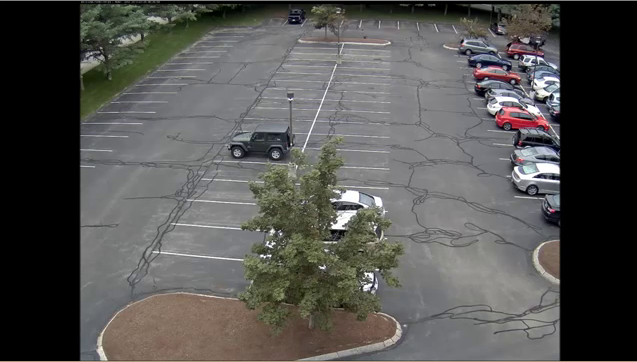
\includegraphics[width=.8\linewidth]{MomentoRastro1}
  \caption{}
  \label{rastrosFig:sfig1}
\end{subfigure}\


\begin{subfigure}{.5\textwidth}
  \centering
  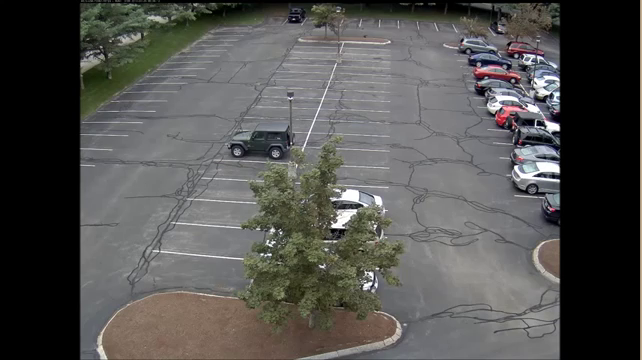
\includegraphics[width=.8\linewidth]{MomentoRastro2}
  \caption{}
  \label{rastrosFig:sfig2}
\end{subfigure}


\begin{subfigure}{.5\textwidth}
  \centering
  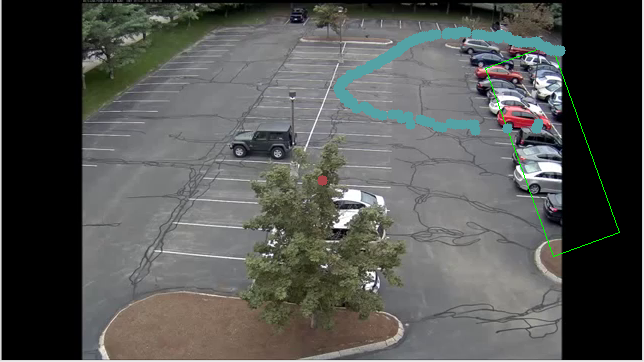
\includegraphics[width=.8\linewidth]{Rastro}
  \caption{}
  \label{rastrosFig:sfig2}
\end{subfigure}
\caption{(a) Um carro aparecendo na cena ; (b)O mesmo carro estacionado em uma vaga; (c) O rastro gerado pelo programa}
\label{rastrosFig}
\end{figure}
      
      
      





\section{Geração de Fundo Dinâmico} \label{geracaoFundo}

     Uma etapa importante do trabalho é a geração de uma imagem de fundo, separada da imagem do vídeo original. Para tal, é preciso implementar um método que separe os elementos do \textit{background} daqueles do \textit{foreground}. Determinamos que os elementos do fundo são aqueles que não estão se movimentando no momento, enquanto os elementos do \textit{foreground} são os objetos que se movem na imagem, em particular, os carros. É importante construir essa imagem, pois é essa segmentação de fundo e plano principal que permitirá mais tarde que o programa determine se uma vaga foi ocupada ou desocupada por um veículo.

     Gerar essa imagem de fundo não é uma tarefa trivial. Devido a própria natureza do espaço sendo filmado, veículos que antes compunham o fundo da imagem podem passar a se mover e veículos que estão em movimento em um determinado momento eventualmente vão estacionar e devem passar a integrar o \textit{background}. É preciso então ter muito cuidado na determinação do fundo do vídeo.

     Antes de mais nada, é preciso determinar uma imagem de fundo inicial. Esse fundo inicial será usado pelo processo de geração dinâmica de fundo descrito mais abaixo. A imagem de fundo base é construída no momento da instalação do \textit{software} deste trabalho, e pode ser reconstruída sempre que desejado, como no início do dia ou no horário que as atividades do estacionamento se iniciam.

     A imagem de fundo inicial \textit{Fi} é formada usando os 30 primeiros quadros capturados em vídeo a partir do momento que sua formação se inicia. O valor de cada \textit{pixel} \textit{i} na imagem tem valor igual a média do valor desse \textit{pixel} em cada um desses quadros, calculada por:

     \begin{equation}\label{mediaFundoInicial}
       V_{i} = \frac{1}{30}\sum_{t=1}^{30}V_{it}
     \end{equation}

     Onde $V_{i}$ é o valor do \textit{pixel} \textit{i} em \textit{Fi} e $V_{it}$ é o valor do \textit{pixel} \textit{i} no frame de número \textit{t}.

     Uma vez obtida \textit{Fi} não podemos simplesmente utilizá-la como um fundo definitivo. A determinação do \textit{background} deve ser feita de forma dinâmica e constante por conta de diversos fatores. Alguns deles são:

     \begin{itemize}
       \item Mudanças na iluminação: com o passar do dia, tanto a iluminação natural quanto a artificial sofrem mudanças. Essas alterações podem fazer com que a cor do asfalto percebida pela câmera mude. É importante adaptar o fundo para que isso não surja como uma diferença entre dois quadros consecutivos
       \item Comportamente dos carros: veículos anteriormente parados podem começar a se mover e veículos em movimento vão estacionar. É preciso adaptar o \textit{background} a esses eventos.
       \item Ruído da câmera: um fundo adaptativo e dinâmico minimiza os problemas causados por ruído na captação do vídeo.
     \end{itemize}

     Para atualizar corretamente o fundo do vídeo, precisamos primeiramente determinar a região do \textit{foreground} da imagem. Para tal, o programa utiliza a imagem D obtida na seção \ref{segmentacaoVeiculos}. A versão binarizada de D passa por uma operação de dilatação que transforma o carro segmentado em uma mancha branca. Essa mancha representa uma região onde o programa sabe com certeza que existe um carro em movimento e será usada como uma máscara para a geração dinâmica do fundo. Chamaremos essa máscara de \textit{Fg}.

     O programa usa essa máscara para atualizar a imagem de fundo para um estado mais apropriado. Para cumprir essa tarefa, primeiro é extraída uma imagem \textit{T} que contém apenas o conteúdo do fundo atual na região da mancha branca \textit{Fg}. Em seguida, \textit{Fg} é invertida e se torna uma mancha preta sobre um fundo branco, chamada \textit{Fg'}. Essa segunda máscara é utilizada para apagar do quadro atual a região de \textit{foreground} determinada pela mancha preta. Em seguida os valores dos pixels diferentes de zero em \textit{T} são inseridos nos pixels da mancha negra sobre a imagem do quadro atual. A média aritmética da soma dos demais valores da imagem do quadro atual e do fundo atual é extraído passa a ser o valor desses pixels no novo fundo.

     O processo inteiro é mais facilmente compreendido através da equação que o define:

     \begin{equation}\label{geracaoFundoEquacao}
       Bgi = \left\{
        \begin{array}{l l}
        Ba_{i} & \text{,Fgi=255} \\
        \frac{Bai}{2} + \frac{Qi}{2} & \text{,Fgi=0}\\
         \end{array} \right.
     \end{equation}

     Onde $Bg_{i}$ é o valor do \textit{pixel} \textit{i} na nova imagem de fundo, $Ba_{i}$ é o valor do \textit{pixel i} na imagem de fundo anterior, $Fg_{i}$ é o valor deste mesmo \textit{pixel} em \textit{Fg} e $Q_{i}$ no quadro atual. Resumidamente, o processo mantém os valores do fundo anterior nos pontos onde se tem certeza que existe um elemento do \textit{foreground} e faz uma média entre o fundo anterior e o quadro atual para os demais valores. A figura \ref{fig:GeracaoFundo} ilustra o processo da geração dinâmica de fundo.


    \begin{figure}
      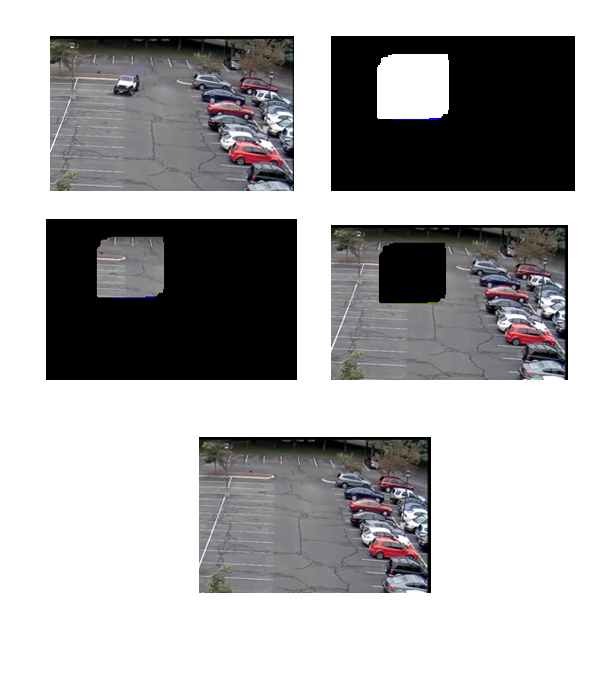
\includegraphics[width=1\textwidth]{FiguraFundo}
      \caption{Imagens representando o processo de geração do fundo dinâmico. No topo o quadro do vídeo e a máscara obtida. No centro a imagem do fundo anterior na região da máscara e a média entre os valores do quadro atual e do fundo anterior nos outros pontos e abaixo o fundo novo construído. }\label{fig:GeracaoFundo}
    \end{figure}

    A imagem de fundo obtida através do processo que foi descrito nessa seção é o objeto de estudo mais importante deste trabalho. Através dela são obtidas as informações relevantes para cumprir os objetivos desejados. Um objeto que aparece na imagem de fundo, é um objeto que parou de se mover e passou a ser um elemento estático do ambiente que está sendo filmado. No contexto do trabalho, isso significa que provavelmente um veículo estacionou. A região obtida pela subtração do fundo em momentos diferentes indica a posição de novos objetos estáticos. Esse processo é descrito na seçõa \ref{diferencasFundos}.





\section{Diferenças entre fundos} \label{diferencasFundos}

    Como foi mencionado ao final da seção \ref{geracaoFundo}, o programa identifica que um objeto que estava em movimento passou a estar parado quando este objeto aparece na imagem de fundo do vídeo. Analogamente, é possível identificar que um objeto que estava parado passou a se mover quando ele desaparece do \textit{background} dinâmico. Fica clara então a importância de se reconhecer quando elementos são adicionados ou removidos do fundo.

    Para identificar mudanças significativas na imagem de fundo do vídeo sendo observado, este programa utiliza o processo de subtração de imagens descrito na seção \ref{subtracao} com algumas modificações. A $t$ quadros do vídeo - onde $t$ é um valor determinado na etapa de calibração do sistema - o programa gera uma imagem de diferença entre o \textit{background} atual e o \textit{background} a $t$ quadros atrás. Essa imagem $Df$ de diferença é obtida através do mesmo processo utilizado para se obter a imagem $D$ de diferença entre dois \textit{frames} na seção \ref{segmentacaoVeiculos}. Essa imagem é submetida a um processo de fechamento, ou seja, a aplicação de uma erosão seguida de uma dilatação. Essa operação tem como objetivo uniformizar os contornos na imagem $Df$ e pricipalmente, eliminar manchas que são pequenas demais para serem consideradas. Por causa disso, a escolha do elemento estruturante para a erosão nessa etapa é muito importante. Esse elemento é o parâmetro que discerne entre os contornos relevantes e os irrelevantes em $Df$.

    Depois que os contornos que não são de interesse para o programa são eliminados de $Df$ é preciso submeter a imagem por um processo de limiarização para que ela seja compatível com as técnicas que serão aplicadas em seguida. Se a imagem do vídeo tem apenas um canal, o \textit{thresholding} aplicado é trivial, cada ponto que não é preto da imagem se torna branco, e os outros continuam pretos como antes. Quando o vídeo possue três canais, é preciso aplicar essa limiarização em cada canal e depois criar uma única imagem binária com as informações de cada canal através da operação lógica \textit{or}. Essa operação faz com que um determinado ponto da imagem resultando seja branco se o ponto de uma das duas imagens sendo operadas for branco e preto caso contrário. Ela é descrita pela equação \ref{equacaoOr}:


    \begin{equation}\label{equacaoOr}
       Or(x,y) = \left\{
        \begin{array}{l l}
        A(x,y) & \text{,A(x,y)=255} \\
        B(x,y) & \text{,B(x,y)=255}\\
        0 & \text{, A(x,y) = 0 e B(x,y) = 0} \\
         \end{array} \right.
     \end{equation}

     Onde $Or(x,y)$ é o valor do \textit{pixel} na posição $(x,y)$ da matriz resultante e $A(x,y)$ e $B(x,y)$ são os valores dos \textit{pixels} nas duas matrizes sobre as quais a operação está sendo aplicada.

     O resultado dessa operação sobre as imagens de binarizadas dos canais R,G e B dois a dois é uma imagem completamente preta, exceto por manchas brancas que representam regiões onde houve uma diferença entre os fundos nos dois momentos. Nessas regiões se pode assumir que ou um objeto novo se integrou ao fundo ou um objeto que antes fazia parte do \textit{background} deixou de fazer.

\section{Identificação de objetos no fundo} \label{identificacaoFundo}

    Apenas encontrar as regiões aonde houve uma diferença entre os fundos não é suficiente para atingir os objetivos do trabalho. Apesar destas regiões indicarem bem precisamente os locais da imagem onde um objeto apareceu ou desapareceu no fundo, elas não são capazes de fornecer algumas informações cruciais. Por exemplo, como saber se uma determinada mancha em $Df$ representa um novo objeto no fundo ou um carro que saiu de uma vaga aonde estava estacionado? Como determinar se o objeto que causou essa diferença sequer é um veículo? É preciso então voltar a analisar as informações contidas na imagem original do quadro do vídeo para identificar corretamente o que está acontecendo na região indicada. Dessa vez porém, o programa pode analisar apenas as pequenas regiões correspondentes àquelas em $Df$.

    Para responder a primeira pergunta apresentada no parágrafo anterior, o programa se utiliza de uma comparação de histogramas. Primeiramente é preciso extrair um histograma de uma região da imagem que seja suficientemente semelhante a uma vaga vazia. Esse histograma $H_{0}$ serve como um histograma de "controle", é o histograma que indica uma vaga vazia. É importante determinar $H_{0}$ de forma dinâmica, a fim de evitar que mudanças na iluminação do vídeo causem resultados incorretos. Para isso, o programa extrai esse histograma em intervalos de tempo regulares, de um espaço na imagem onde é sabido que não há carros. A determinação desse espaço pode ser feita manualmente no momento de instalação do programa ou posteriormente através de uma função de calibração. É importante escolher uma região onde ocorrem muito poucas mudanças na imagem de fundo e que seja semelhante ao fundo da imagem sem nenhum elemento. Em outras palavras, para o caso desse programa, deve-se escolher uma região que representa o chão do estacionamento e que não se espera que seja ocupada por objetos.

    Munido com $H_{0}$ o programa extrai o histograma $H_{1}$ da área do fundo atual correspondente à cada mancha branca presente em $Df$. Em seguida o histograma $H_{2}$ da mesma região no fundo a $t$ quadros atrás é extraído.  O programa faz uma comparação entre $H_{1}$ e $H_{2}$. Se os histograma forem suficientemente distintos, é considerado que houve uma mudança significativa no \textit{background}. Nesse caso, o programa compara $H_{1}$ e $H_{2}$ com $H_{0}$. Essa segunda comparação tem como objetivo determinar se um objeto foi adicionado ou removido do fundo. Quando o $H_{1}$ é semelhante a $H_{0}$, pode-se assumir que a região observada mostra uma vaga vazia. Por outro lado, quando $H_{2}$ é semelhante a $H_{0}$, é muito provável que a região observada mostra um objeto novo que se integrou ao fundo.

    Os histogramas são comparados através de um pequeno conjunto de parâmetros. Os parâmetros escolhidos não podem ser estritamente dependentes do tamanho da região analisada, já que não há garantia de que a região de controle terá o mesmo tamanho da região indicada em $Df$. O primeiro desses parâmetros é o nível de cinza que ocorre com mais frequência na região. Esse parâmetro é suficiente para determinar se as áreas analisadas são diferentes demais umas das outras, uma vez que imagens com níveis de cinza predominante demasiado diferentes certamente serão consideravelmente distintas. Porém, não se pode assumir o contrário, que uma coincidência nesse valor indica imagens semelhantes. Para complementar esse parâmetro o programa usa a técnica de intersecção detalhada na seção \ref{comparacaoHistogramas}. Se dois histogramas apresentam um valor muito alto de intersecção, é muito provável que essas duas imagens sejam parecidas.

    A figura \ref{DiferencaHistogramaFig} mostra esses dois histogramas para os dois momentos representados na figura \ref{SubtracaoFig}. Nela é visível a diferença da distribuição dos valores de cinza na imagem.


\begin{figure}
 \centering
\begin{subfigure}{.5\textwidth}
  \centering
  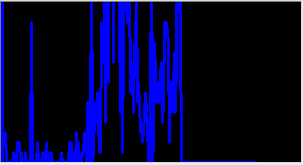
\includegraphics[width=.8\linewidth]{HistogramaFundo}
  \caption{}
  \label{DiferencaHistogramaFig:sfig1}
\end{subfigure}\


\begin{subfigure}{.5\textwidth}
  \centering
  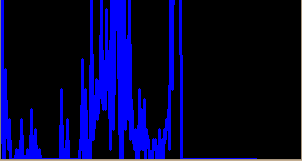
\includegraphics[width=.8\linewidth]{HistogramaFundoAnterior}
  \caption{}
  \label{DiferencaHistogramaFig:sfig2}
\end{subfigure}
\caption{(a) O histograma $H_{1}$ da figura \ref{Subtracao:sfig1} na área indicada por \ref{Subtracao:sfig3}; (b)O histograma $H_{2}$ da figura \ref{Subtracao:sfig2} na área indicada por \ref{Subtracao:sfig3}}
\label{DiferencaHistogramaFig}
\end{figure}

\section{Verificação de objetos no fundo}\label{verificaoObjetosFundo}

    Uma vez determinado que um objeto novo se integrou ao fundo da imagem, é preciso garantir então que o objeto que se integrou ao fundo na posição da vaga é realmente um veículo. O sistema não deve acusar que uma vaga foi ocupada quando algum outro corpo está sobre a vaga, como por exemplo uma pessoa que interrompeu seu trajeto sobre uma vaga ou a porta de um carro na vaga adjacente que ficou aberta por muito tempo. Observe que esse cuidado e suficiente para garantir que o sistema não libere vagas incorretamente quando um objeto que não é um carro sai dessa vaga, uma vez que a vaga nunca é marcada como ocupada nesse caso.

    Para identificar o objeto novo que apareceu no fundo da imagem, o sistema se utiliza pricipalmente de um recurso, a comparação da posição de um objeto identificado com os finais dos rastros identificados na seção \ref{rastreamentoVeiculos}. Antes de afirmar que uma vaga foi ocupada por um veículo quando identifica uma mudança no fundo sobre a área de uma vaga, o programa percorre o vetor de rastros obtidos e identifica se algum deles tem início em um ponto fora de qualquer vaga e o final dentro da região do objeto identificado. Se esse for o caso, garante-se que esse objeto que apareceu estava anteriormente em movimento. Isso significa que a diferença na região não foi causada por um objeto que surgiu subitamente na cena naquela posição, como um grande pico de ruído, uma porta que se abriu em um carro adjacente ou alguma mudança de cor sobre um carro parado, possivelmente causada por um vidro abrindo ou o reflexo de uma luz.

    Como um complemento a esse recurso, o programa se utiliza de um algoritmo simples de classificação para determinar a probabilidade de que o objeto seja de fato um carro. Esse algoritmo usa informações sobre as bordas presentes nas imagens para diferenciar principalmente veículos de pessoas. Características utilizadas para esse sistema de classificação incluem a largura, o comprimento, quanto uma determinada cor ocupa no objeto e a presença de alguns componentes como pára-brisas que ajudam a confirmar que o objeto é um veículo. Esse sistema será descrito com mais detalhes posteriormente.






  \chapter{Resultados Parciais}\label{resultados}

\section{Testes em imagens estáticas} \label{testesEstaticas}

Os primeiros testes aplicados no programa foram feitos com imagens estáticas ao invés de imagens de vídeo. O propósito destes testes era verificar a eficácia do algoritmo de diferenciação de fundos detalhado na seção \ref{diferencasFundos}. Cada imagem estática fazia o papel de uma imagem de fundo que teria sido extraída de um vídeo da câmera no estacionamento. As imagens para os primeiros testes foram obtidas com o auxílio de um \textit{drone} de controle remoto que fez fotografias aéreas do estacionamento próximo aos prédios PAT e PJC no campus da Universidade de Brasília. A fim de simular melhor a imagem que seria obtida por uma câmera instalada em um poste no estacionamento, um programa de edição de imagens foi utilizado para recortar pedaços da imagem com um nível maior de aproximação. Essas foram as imagens utilizadas para os testes.

A primeira etapa dessa bateria de testes foi testar o caso mais simples de todos: comparar uma imagem de fundo com a imagem do estacionamento completamente desocupado. Através de manipulação de imagens, foram compostas diversas imagens com carros de cores diferentes, estacionados em várias combinações distintas de vagas. Cada imagem é comparada a imagem da seção de estacionamento correspondente com todas as vagas desocupadas. Aqui, uma diferença entre as duas imagens que esteja em uma região que se sabe que é uma vaga sempre representa um carro que passou a ocupar aquela vaga. Uma terceira imagem mostra através de círculos coloridos quais vagas estão ocupadas na imagem de teste.  Nessa etapa de testes, o programa obteve uma taxa de acerto de 100\%. A figura \ref{ComparacaoFundoVazioFig} mostra alguns resultados desses testes.

O bom funcionamento nesse caso simples é de grande importância. Se o programa for inicializado com o estacionamento vazio, a primeira comparação de fundo será dessa maneira. Se o algoritmo acerta quais vagas estão ocupadas, ele agora está munido da informação completa dos estados das vagas. A partir desse momento, é possível interpretar de forma mais simples as diferenças na imagens de fundo obtidas no vídeo. Uma diferença significativa sobre uma região de vaga livre, significa que a vaga foi ocupada. Se a vaga estava ocupada, ela foi liberada entre uma verificação e outra. Assim, o algoritmo consegue indicar o estado das vagas com uma taxa muito alta de acerto através de operações simples, desde que o estado inicial seja conhecido.

\begin{figure}
 \centering
\begin{subfigure}{.5\textwidth}
  \centering
  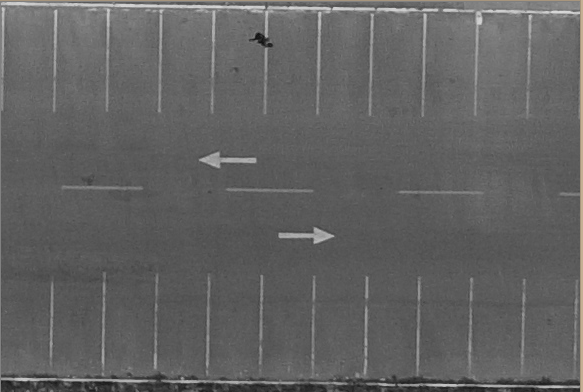
\includegraphics[width=.8\linewidth]{Vazio}
  \caption{}
  \label{ComparacaoFundoVazioFig:sfig1}
\end{subfigure}\

\begin{subfigure}{.5\textwidth}
  \centering
  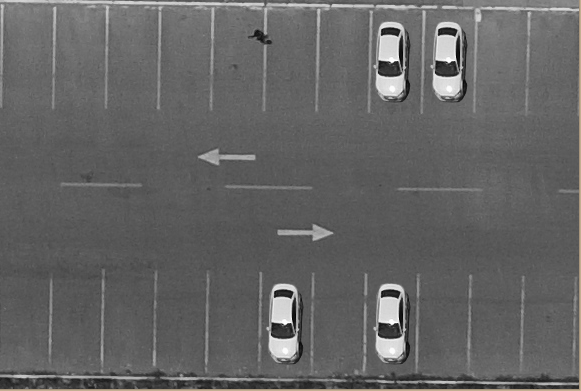
\includegraphics[width=.5\linewidth]{4Carros}
  \caption{}
  \label{ComparacaoFundoVazioFig:sfig2}
\end{subfigure}%
\begin{subfigure}{.5\textwidth}
  \centering
  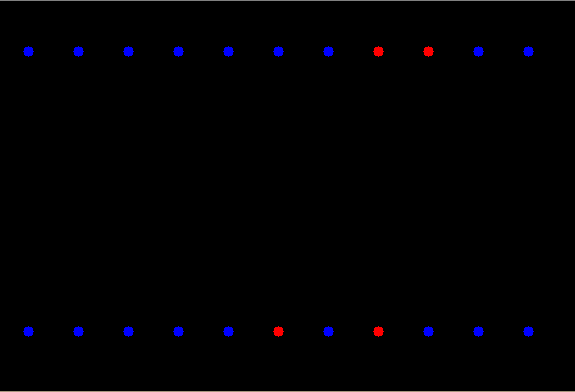
\includegraphics[width=.5\linewidth]{Indicacao4Carros}
  \caption{}
  \label{ComparacaoFundoVazioFig:sfig3}
\end{subfigure}

\begin{subfigure}{.5\textwidth}
  \centering
  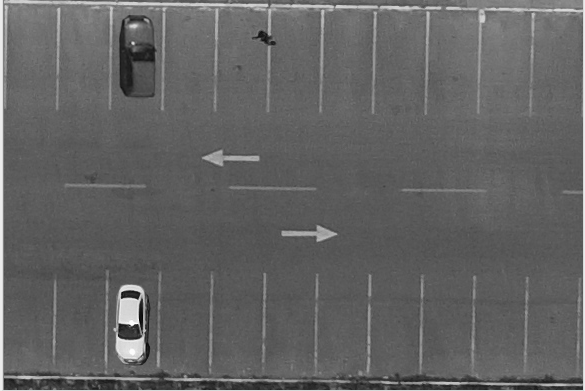
\includegraphics[width=.5\linewidth]{2Carros}
  \caption{}
  \label{ComparacaoFundoVazioFig:sfig4}
\end{subfigure}%
\begin{subfigure}{.5\textwidth}
  \centering
  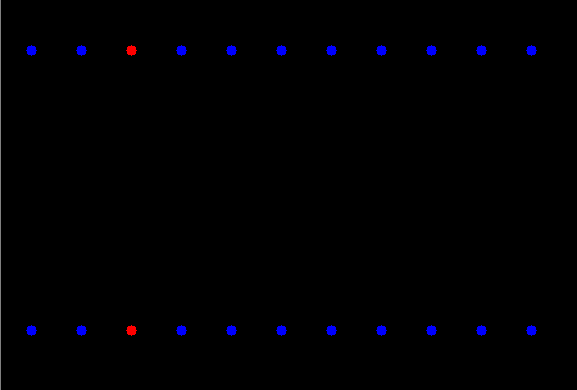
\includegraphics[width=.5\linewidth]{Indicacao2Carros}
  \caption{}
  \label{ComparacaoFundoVazioFig:sfig5}
\end{subfigure}



\caption{(a) O estacionamento vazio; (b) Quatro carros estacionados; (c) As indicações de ocupação das vagas em (b); (d) Dois carros estacionados; (e) As indicações dos estados das vagas em (d)}
\label{ComparacaoFundoVazioFig}
\end{figure}

Infelizmente, nem sempre se conhece o estado inicial do vetor de vagas quando o algoritmo começa a executar. Ele pode ter sido iniciado sobre um estacionamento que não estava completamente vazio ou a câmera ter sido desligado durante sua execução. Nesse caso o programa precisa ser capaz de determinar o estado das vagas a partir de uma determinada imagem do vídeo, normalmente uma imagem de fundo para a partir daí poder utilizá-lo para as avaliações futuras. Além disso, é preciso utilizar as técnicas apresentadas nas seções \ref{identificacaoFundo} e \ref{verificaoObjetosFundo} para evitar falsos positivos.


Por causa disso, a segunda etapa de testes consiste na comparação de duas imagens de fundo de momentos diferentes. O programa deve então ser capaz de utilizar as técnicas apresentadas e determinar corretamente o estado de ocupação das vagas sem se utilizar do conhecimento prévio do estado anterior. Para realizar essa tarefa, o programa verifica novamente as diferenças nas vagas. Nas regiões onde houve diferença, como aquela indicadas na figura \ref{regioesDiferencaTesteFig} o programa faz a comparação de histograma com o estado anterior para determinar se o movimento foi de chegada ou saída de um veículo. Se utilizando dessa comparação o programa atualiza o vetor dos estados das vagas. Os estados das vagas onde não houve diferença pode ser determinado por classificação de objetos ou também por uma comparação de histogramas, basta comparar o histograma com o de controle ou com o de uma vaga que acabou de ser desocupada.


\begin{figure}
 \centering
 \begin{subfigure}{.5\textwidth}
  \centering
  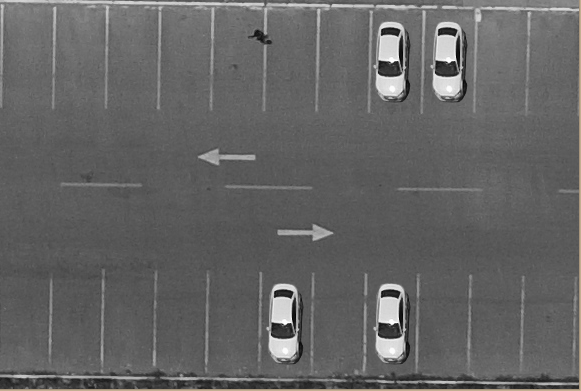
\includegraphics[width=.5\linewidth]{4Carros}
  \caption{}
  \label{regioesDiferencaTesteFig:sfig1}
\end{subfigure}%
\begin{subfigure}{.5\textwidth}
  \centering
  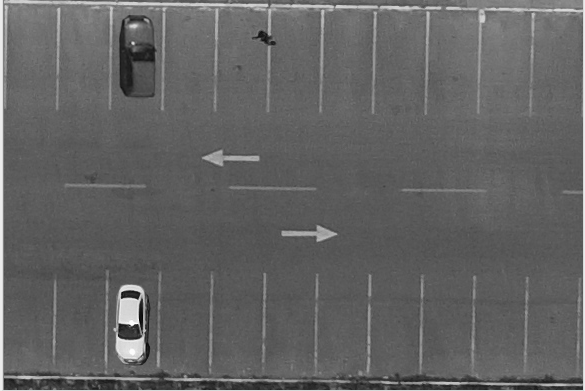
\includegraphics[width=.5\linewidth]{2Carros}
  \caption{}
  \label{regioesDiferencaTesteFig:sfig2}
\end{subfigure}

 \begin{subfigure}{.5\textwidth}
  \centering
  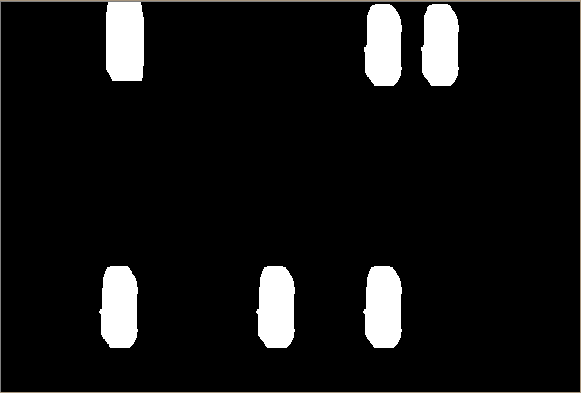
\includegraphics[width=.8\linewidth]{Diferenca4-2Carros}
  \caption{}
  \label{regioesDiferencaTesteFig:sfig3}
\end{subfigure}%


\caption{(a) Quatro carros estacionados; (b) Dois carros estacionados; (c) As manchas que indicam aonde houve diferença entre as duas imagens.}
\label{regioesDiferencaTesteFig}
\end{figure}

Apesar das indicações de diferença parecerem muito precisas, nenhum dos métodos de comparação de histograma apresentados na subseção \ref{comparacaoHistogramas} foi suficiente para que o programa tivesse uma taxa de acerto satisfatória até agora, mas ela tem aumentado a cada nova versão do programa. Esse algoritmo vai continuar a ser aprimorado para as próximas etapas do trabalho. A tabela \ref{tabelaDiferencasHistogramas} mostra os valores obtidos pela diferença $\chi^2$ e pelo cálculo de intersecção das vagas com o histograma de controle, e a figura \ref{histogramasRegioesPequenas} mostra os histogramas de cada uma delas e o histograma de controle.

Analisando essa tabela e as imagens dos histogramas, pode-se perceber que os valores obtidos não são suficiente para se determinar um limiar de semelhança com nenhuma das duas técnicas ainda. Imagens semelhantes estão apresentando um distância maior do que o esperado. O maior fator impeditivo é a grande disparidade entre os valores das vagas 4 e 5, que estão ambas vazias e deveriam mostrar valores similares quando comparadas ao histograma de controle.


\begin{figure}
 \centering
 \begin{subfigure}{\textwidth}
  \centering
  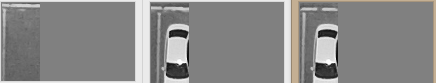
\includegraphics[width=\linewidth]{RegioesPequenas1}
  \caption{}
  \label{regioesPequenasTesteFig:sfig1}
\end{subfigure}%

\begin{subfigure}{\textwidth}
  \centering
  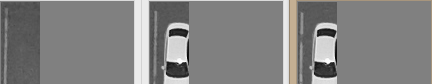
\includegraphics[width=\linewidth]{RegioesPequenas2}
  \caption{}
  \label{regioesPequenasTesteFig:sfig2}
\end{subfigure}


\caption{As diferentes regiões da imagem de fundo que são analisadas no caso apresentado na figura \ref{regioesDiferencaTesteFig}. Na parte superior da esquerda para a direita: vagas 5, 15 e 17. Na parte inferior vagas 4, 10 e 14.}
\label{regioesPequenasTesteFig}
\end{figure}


\begin{figure}
 \centering
  \begin{subfigure}{.3\textwidth}
  \centering
  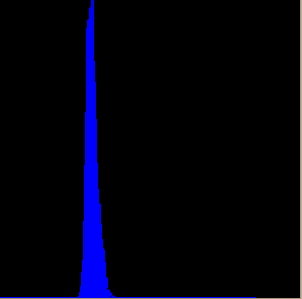
\includegraphics[width=.8\linewidth]{HistogramaControle}
  \caption{}
  \label{histogramasRegioesPequenasFig:sfig1}
\end{subfigure}%


 \begin{subfigure}{.8\textwidth}
  \centering
  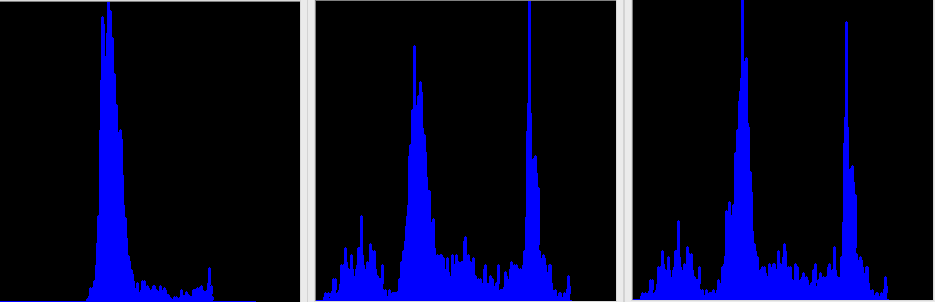
\includegraphics[width=.5\linewidth]{histogramasTesteSuperior}
  \caption{}
  \label{histogramasRegioesPequenasFig:sfig1}
\end{subfigure}%

\begin{subfigure}{.8\textwidth}
  \centering
  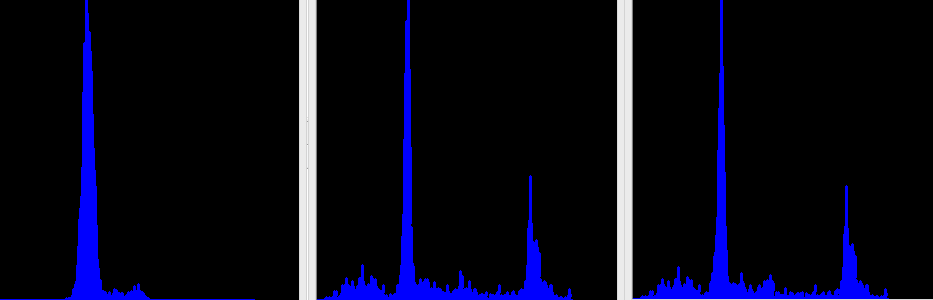
\includegraphics[width=.5\linewidth]{histogramasTesteInferior}
  \caption{}
  \label{histogramasRegioesPequenasFig:sfig2}
\end{subfigure}


\caption{(a)O histograma de controle; (b) Os histogramas das imagens apresentadas em  \ref{regioesPequenasTesteFig:sfig1}; (c) Os histogramas das imagens apresentadas em  \ref{regioesPequenasTesteFig:sfig2};}
\label{histogramasRegioesPequenasFig}
\end{figure}




\begin{table}
\centering
 \begin{tabular}{||c c c||}
 \hline
 Vaga & $\chi^2$ & Intersecção \\ [0.5ex]
 \hline\hline
 4 & 2371.72 & 2442.04 \\
 \hline
 5 & 189588 & 476.993 \\
 \hline
 10 & 15373.5 & 1428.9 \\
 \hline
 14& 8747.21 & 1506.91 \\
 \hline
 15 & 33113.5 & 809.946 \\
 \hline
 17 & 113295 & 474.473 \\ [1ex]
 \hline
\end{tabular}

\caption{A tabela com os valores obtidos pelas duas técnicas de comparação de histograma utilizadas}
\label{tabelaDiferencasHistogramas}
\end{table}




Se acredita que a melhor solução para atingir uma taxa de acerto satisfatória é melhorar a técnica que o programa se utiliza para determinar a região da imagem de fundo original a ser analisada a partir da imagem de diferença \ref{regioesDiferencaTesteFig:sfig3}.Atualmente, o programa determina os contornos da imagem e calcula a partir deles o menor retângulo inclinado $R$ que os contém e em seguida obtém o retângulo aonde $R$ está inscrito. Esse segundo retângulo determina a região da imagem de fundo a ser analisada para cada vaga. Na figura \ref{regioesPequenasTesteFig} pode-se observar que essa técnica obtém regiões que não são completamente precisas. Essa falha atrapalha a medição e gera resultados indesejados. A solução que está sendo explorada envolve adaptar a região contida em $R$ para que ela apareça sem inclinação em uma outra imagem, facilitando a análise e aumentando a precisão dos resultados.

Outra solução que possivelmente aumentará a precisão dos resultados é converter cada fração da imagem de fundo que está sendo analisada para o formato HSV, que é a representação mais natural da visualização de imagens, e fazer a comparação de histogramas normalizados do canal H dessas imagens. Essa mudança é a próxima etapa do trabalho e se acredita que pode ser um ponto crucial na sua implementação, uma vez que aumentar a taxa de acerto nessa etapa permite avançar para a próxima etapa de implementação.

\section{Primeiros testes em vídeos}\label{testesVideos}

A outra parcela de testes que já foi executada sobre o programa utilizou vídeos adquiridos \textit{online}. Foram utilizados vídeos da internet por causa da dificuldade de se obter filmagens úteis nesse momento da execução do trabalho. O propósito dessa etapa de testes era avaliar o funcionamento do algoritmo de geração dinâmica de \textit{background} exposto na seção \ref{geracaoFundo} e experimentar com o algoritmo de rastreamento descrito na seção \ref{rastreamentoVeiculos}. Por causa da natureza e do propósito dos testes, algumas das filmagens utilizadas nesse momento não são de estacionamentos, uma vez que nesse etapa não se fazia totalmente necessário que as imagens analisadas fossem completamente coerentes com aquelas que virão a ser analisadas pelo programa no futuro. Em um momento posterior da implementação do trabalho, pretende-se gerar animações através das imagens estáticas utilizadas na seção \ref{testesEstaticas} e filmagens em um modelo em escala de um estacionamento real, para que possam ser feitos testes provisórios antes da etapa de validação do algoritmo.

\subsection{Testes de geração de fundo} \label{testesFundo}

Foram feitos testes do algoritmo de geração dinâmica de fundo (\ref{geracaoFundo}) em um vídeo de uma câmera de um estacionamento e em uma série de vídeos de câmeras de segurança de vias de trânsito obtidos através da internet. Para satisfazer os testes, o algortimo deveria cumprir uma série de condições:
    \begin{itemize}
      \item No vídeo resultante do sistema os objetos em movimento no vídeo original deveriam estar completamente invisíveis ao olho humano.
      \item As regiões de diferença obtidas deveriam estar suficientemente próximas dos objetos em movimento no vídeo original.
      \item O algoritmo deveria ser capaz de integrar objetos que entraram na cena e pararam de se mover ao fundo.
      \item Também deve ser capaz de perceber que objetos antes integrados ao fundo passaram a se mover.
      \item Não deve fazer operações sobre diferenças insignificantes entre dois quadros de vídeo.
    \end{itemize}

A primeira condição apresentada, obviamente, irrelevante para o sistema de computador, mas é um bom indicador para os desenvolvedores do funcionamento do algoritmo e está fortemente ligada ao cumprimento da segundo condição, tendo a vantagem de ser muito mais fácil e intuitiva de se verificar. As condições sobre a mudança de estado de objetos para o fundo são também de fácil verificação, mas são de extrema importância para o trabalho. Se o algoritmo não for capaz de cumprir essas duas condições, ele não é adequado para o sistema que esse projeto visa desenvolver. A última condição é de mais difícil verificação, mas por sorte é também a menos relevante delas, uma vez que existe um mecanismo redundante para eliminiação de regiões de diferença insignificante na etapa de subtração de fundos descrita na seção \ref{testesEstaticas}.

No geral, o algoritmo se mostrou muito capaz de cumprir todas as condições. Apesar de haverem momentos onde o resultado não foi totalmente perfeito, o programa teve desempenho satisfatório sobre as regiões relevantes em todos os vídeos de teste. Durante os testes, percebeu-se que o algoritmo funcionava muito melhor quando tratava de veículos em velocidades maiores e cores mais claras. Isso era de se esperar pela implementação do algoritmo. Objetos que se movem mais rapidamente geram diferenças quadro-a-quadro maiores e por isso a região obtida aonde o programa assume que existe um veículo é mais precisa. Como consequência dessa característica, ao olho humano, veículos que estão desacelerando passam a aparecer gradualmente na vídeo de fundo, a medida que pedaços dele passam a se mover muito pouco para que a diferença seja siginificativa. Isso não interfere na execução do problema, por causa da natureza periódica da subtração entre fundos. Uma escolha correta do intervalo de tempo para subtração e pesos das imagems do quadro inicial e fundo anterior no momento de geração amenizam ainda mais esse aparecimento gradual. Quando um objeto passava a se movimentar o algoritmo sempre era capaz de perceber essa mudança imediatamente, porém, por causa da natureza da geração do fundo, o desaparecimento é gradual. Novamente, um ajuste de parâmetros traz esse problema para níveis aceitávies. A figura \ref{figTestesFundos} demonstram alguns resultados.

\begin{figure}
 \centering
  \begin{subfigure}{.6\textwidth}
  \centering
  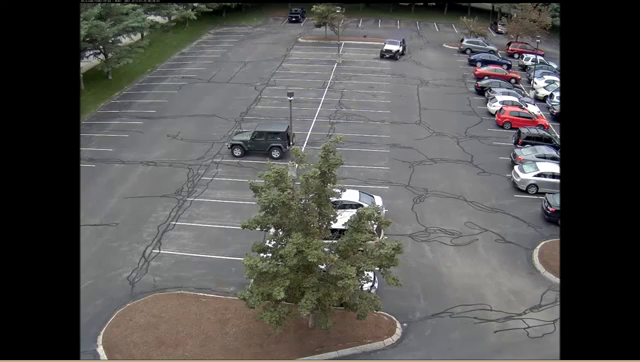
\includegraphics[width=.5\linewidth]{Video}
  \caption{}
  \label{figTestesFundos:sfig1}
\end{subfigure}%
 \begin{subfigure}{.6\textwidth}
  \centering
  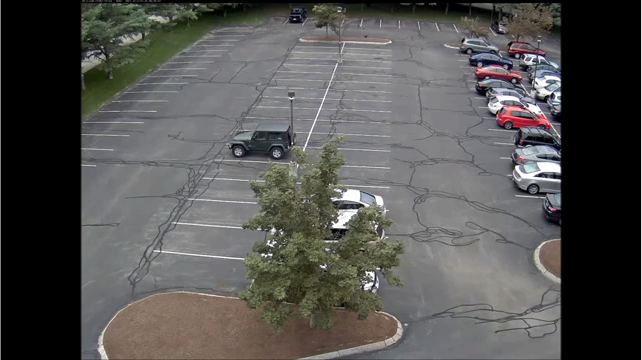
\includegraphics[width=.5\linewidth]{Fundo}
  \caption{}
  \label{figTestesFundos:sfig2}
\end{subfigure}

\begin{subfigure}{.6\textwidth}
  \centering
  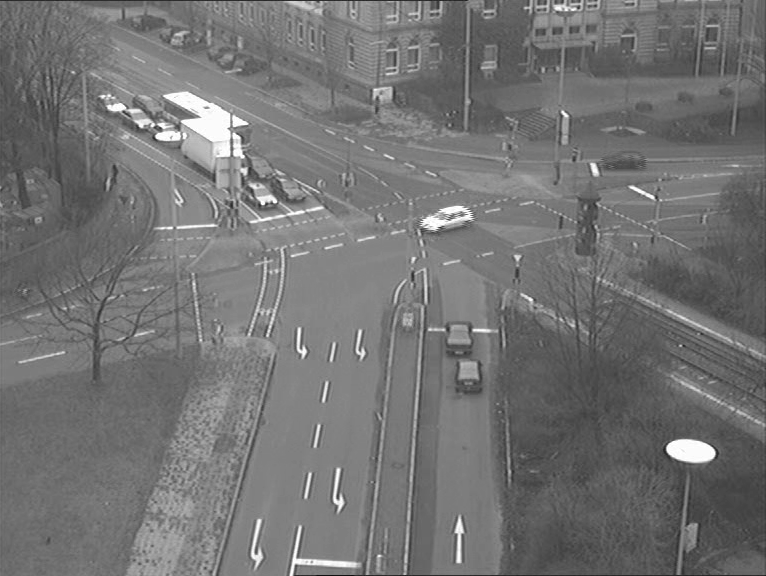
\includegraphics[width=.5\linewidth]{Quadro1}
  \caption{}
  \label{figTestesFundos:sfig3}
\end{subfigure}%
\begin{subfigure}{.6\textwidth}
  \centering
  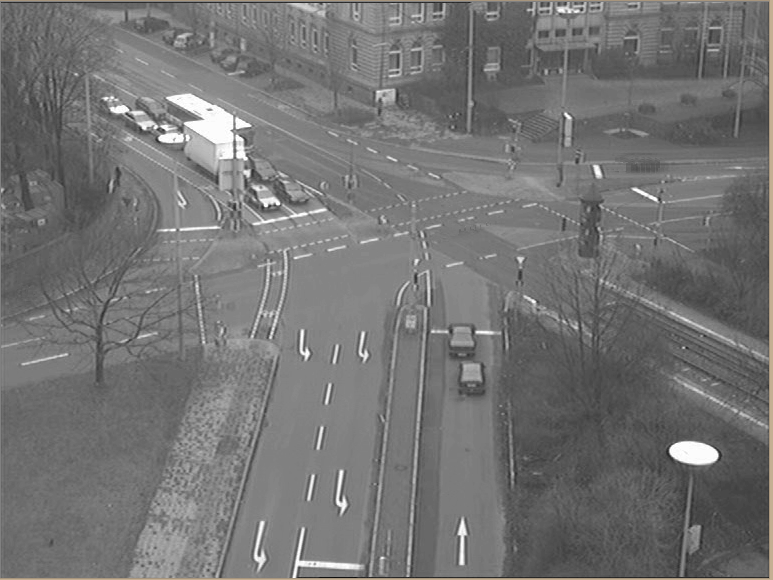
\includegraphics[width=.5\linewidth]{Fundo1}
  \caption{}
  \label{figTestesFundos:sfig4}
\end{subfigure}


\caption{(a) e (b) um quadro do vídeo de um estacionamento e o fundo correspondente; (c) e (d) um quadro de um dos vídeos de tráfego e o seu fundo correspondente.}
\label{figTestesFundos}
\end{figure}


Para a verificação da última condição a saída do algoritmo foi modificada. Ao invés de retornar um vídeo contendo apenas a imagem do fundo, para esses testes o algoritmo mostrava na tela um vídeo de um fundo completamente preto, exceto pelas regiões de \textit{foreground}. Dessa forma era possível avaliar quais regiões estavam sendo consideradas como suficientemente diferentes para o algoritmo. Esses testes mostraram que em imagens com pouco ou nenhum ruído, o mecanismo apresentado de eliminição de pequenas regiões funciona com 100\% de satisfação. Apenas as regiões com objetos em movimento eram mostradas na saída de vídeo. Em imagens muito ruidosas porém, percebeu-se que é necessário um tratamento prévio, a fim de eliminar o ruído presente. É preciso então avaliar métodos de remoção de ruído de imagens e determinar um que seja capaz de eliminar as impurezas indesejadas sem interferir na detecção dos objetos em movimento. A figura \ref{testeSegmentacaoFig} mostra a saída dessa forma do quadro mostrado na figura \ref{figTestesFundos:sfig3}. Nela pode-se perceber um pequeno erro causado por ruído e falhas na segmentação do carro preto no canto superior direito da tela.

\begin{figure}
 \centering
  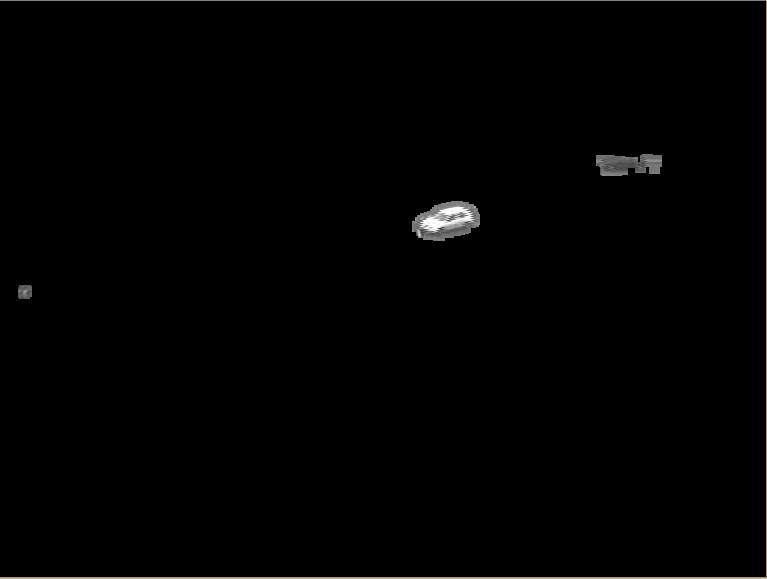
\includegraphics[width=.5\textwidth]{Seg1}  
    \caption{A segmentação do algoritmo de geração de fundo quadro na figura \ref{figTestesFundos:sfig3}.}
\label{testeSegmentacaoFig}
\end{figure}

Ao fim destes testes, se concluiu que o algoritmo da forma como está implementado agora cumpre satisfatoriamente as necessidades impostas pelo programa e é completamente adequado para as tarefas exigidas para o seu funcionamento. O algoritmo mostrou resultados excelentes em geração de fundo para veículos em velocidade moderada e se movendo continuamente. Ainda é também capaz de integrar corretamente ao fundo da imagem qualquer objeto que interrompa seu movimento por tempo suficiente. Acredita-se ainda que esse algoritmo seja útil em diversos outros trabalhos. Por exemplo, com poucos ajustes o algoritmo seria perfeitamente capaz de detectar veículos que estejam se movimento sobre uma rodovia e poderia ser usado em programa de análise de fluxo de tráfego.

\subsection{Testes do sistema de rastreamento} \label{testesRastreamento}

Para os testes do sistema descrito na seção \ref{rastreamentoVeiculos}, foi usado apenas o vídeo que contém a filmagem do movimento em um estacionamento. Vídeos de câmera de tráfego em ruas tornavam a análise muito difícil em razão do elevado número de rastros gerados. Obviamente, mais testes serão elaborados posteriormente, quando filmagens mais adequadas forem obtidas.

As análises executadas sobre o resultado desse sistema forem principalmente visuais, de forma que o resultado era analisado através de observação humana da imagem resultante do processo. A preocupação principal nesses testes era a corretude das posições dos círculos desenhados no rastro e a identificação correta da posição relativa entre o início e o fim dos rastros e o interior de vagas, verificado através de informação exibida na saída padrão do computador pelo programa.

É de extrema importância que o programa seja capaz de identificar que um rastro representa um trajeto que teve início fora de uma vaga e final no seu interior. Não apenas isso, é crucial que ele não acuse falsos positivos no caso de um veículo passar rapidamente por dentro de uma região que representa uma vaga mas não estacionar. Essa detecção é parte do mecanismo de verificação do estado das vagas, juntamente com a subtração dos fundos em momentos distintos.

Os testes sobre o vídeo em questão mostraram que o sistema é totalmente capaz de detectar e desenhar corretamente na tela de saída um rastro que representa o trajeto de veículos em movimento no estacionamento. Além disso, as condições e parâmetros para decidir se um contorno de diferença faz parte do trajeto se mostraram suficientes e corretos. Também se observou uma taxa total de acertos na posição relativa entre os pontos inicias e finais e o interior das vagas. Porém, o programa apresentou alguns defeitos nessa etapa. Diferenças pequenas na imagem, causadas por ruído ou movimentos pequenos em uma região geravam rastros muito curtos, algumas vezes com um só ponto. Apesas desses rastros não representarem um problema muito siginificante nesse momento, porque na grande maioria dos casos vão se iniciar e terminar em ponto quase iguais e não vão acusar que houve movimento para dentro ou fora de uma vaga, reconhece-se que eles são indesejados e a aparição deles não é uma situação ideal e é potencialmente perigosa para o bom funcionamento do programa. A figura \ref{testesRastrosFig} mostra dois rastros em um vídeo. Na figura os pequenos rastros problemáticos são visíveis na região da árvore.

\begin{figure}
 \centering
  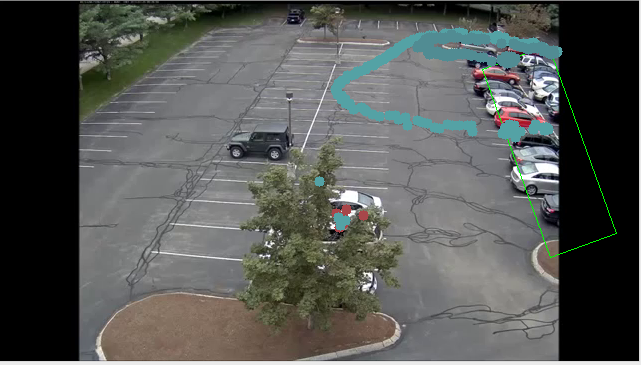
\includegraphics[width=.5\textwidth]{2Rastros}
    \caption{O rastro de dois carros em um vídeo de um estacionamento.}
\label{testesRastrosFig}
\end{figure}

Concluiu-se então que é preciso refinamento nesse componente do programa. Apesar do algoritmo utilisado atualmente ser capaz de mostrar visualmente um rastro de um veículo com bastante precisão, ele apresenta diversos riscos para falsos positivos que não devem ser desconsiderados na implementação final do programa. Métodos diferentes de rastreamento e outras alternativas já estão sendo estudados para implementação.



  \chapter{Considerações finais}

O programa ainda está em um estado inicial, no qual ainda estão sendo desenvolvidos componentes básicos para a implementação do programa em si e os testes estão sendo feito sobre funções específicas. Nessa etapa o foco foi em adquirir o conhecimento necessário para a implementação final e explorar opções que podem vir a ser usadas no programa definitivo. Várias técnicas foram estudadas e testadas, várias ainda estão sendo. Ainda há um elemento de exploração de possibilidades nessa etapa da implementação do trabalho.

Durante esse tempo de testes, concluiu-se que implementar um projeto completo com o escopo indicado é definitivamente viável, tanto técnicamente quanto conceitualmente. A abordagem tomada até o momento também parece estar na direção correta. Sendo assim, o projeto continuará no caminho que está sendo tomado atualmente, com previsão de término em pouco tempo.

As etapas futuras de implementação envolvem mais testes em imagens artificais, criadas especificamente para o trabalho, como fotografias e animações manipuladas através de programas de edição de imagens, simulando diversas condições de ambiente, luz e clima para que seja feita uma pré-validação das funcionalidades separadamente e depois como um todo antes de se iniciarem os testes em com imagens reais e em tempo real.

Espera-se que ao final desse trabalho, tenha-se produzido um \textit{software} que atende a todos os objetivos apresentados e que seja capaz de ajudar diversas pessoas de formas distintas e importantes, sendo uma pequena parte da solução de um problema que afeta tanto motoristas comuns quanto donos de estabelecimento comerciais e até metrópoles globais como um todo. Ao término do programa, espera-se também que tenha acontecido ainda mais aprendizado na área de Processamento de Imagens, que continua se mostrando cada vez mais importante no mundo comercial.

 
  % ...

  \postextual
  \bibliographystyle{plain}
  \bibliography{bibliografia}

\end{document}
